\documentclass[conference]{IEEEtran}

% correct bad hyphenation here
%\hyphenation{op-tical net-works semi-conduc-tor}

% packages
\usepackage[dvips]{graphicx}

\usepackage{listings}
\usepackage[cmex10]{amsmath}
\usepackage{url}
\usepackage{caption}
\usepackage{fancyvrb}
\usepackage{upquote}
\usepackage{multicol}
\usepackage{tikz}
\usepackage{scalerel}
\usepackage{longtable}
\usepackage{etoolbox}
\usepackage{float}
\usepackage{amssymb}
\usepackage{mathtools}
\usepackage{subcaption}
\usepackage{booktabs}
\usepackage{multirow}
\usepackage{algpseudocode}
\usepackage{calc,multicol}
\usepackage{algorithm}
\usepackage{setspace}

% page number out of Last page
\usepackage{lastpage}
% \usepackage{fancyhdr}
% \pagestyle{fancy} 
% \fancyfoot[C]{{\thepage} of \pageref{LastPage}}
% \renewcommand{\headrulewidth}{0pt}

\DeclarePairedDelimiter{\ceil}{\lceil}{\rceil}
\DeclarePairedDelimiter\floor{\lfloor}{\rfloor}

% define environments
\patchcmd{\thebibliography}{\clubpenalty4000}{\clubpenalty10000}{}{}
\patchcmd{\thebibliography}{\widowpenalty4000}{\clubpenalty10000}{}{}

% Graphics
\DeclareGraphicsExtensions{.pdf,.jpg,.png}
\graphicspath{ {./img/} }

% New commands
\newcommand{\keywords}[1]{\par\addvspace\baselineskip
\noindent\keywordname\enspace\ignorespaces#1}
\newtheorem{grammar}{Grammar snippet\#}
\let\oldnl\nl% Store \nl in \oldnl
\newcommand{\nonl}{\renewcommand{\nl}{\let\nl\oldnl}}% Remove line number for one line
\newcommand{\sangle}[1]{$\stretchleftright{\langle}{#1}{\rangle}$}
\newcommand{\mcell}[3][c]{%
    \begin{tabular}[#1]{@{}#2@{}}#3\end{tabular}}%
\newcommand{\east}[0]{{\sc EAST-ADL}\xspace}

\newtheorem{remarkex}{Remark}
\newtheorem{remarkreq}{Remark}
\newtheorem{remarkdef}{Remark}

\newtheorem{example}[remarkex]{Example}
\newtheorem{req}[remarkreq]{Req\texttt{\#}}
%\newtheorem{remark}{Remark}[section]
\newtheorem{definition}[remarkdef]{Definition}
\newtheorem{theorem}[remarkdef]{Theorem}
% start of the document
\begin{document}
% first the title is needed
\setstretch{0.93}
\title{Power-aware Allocation of Fault-tolerant Multirate AUTOSAR Applications, this text is added from remote}
% a short form should be given in case it is too long for the running head
\author{
\IEEEauthorblockN{
Nesredin Mahmud\IEEEauthorrefmark{1}, 
Guillermo Rodriguez-Navas\IEEEauthorrefmark{1},
Hamid Faragardi\IEEEauthorrefmark{4},
Saad Mubeen\IEEEauthorrefmark{1},
Cristina Seceleanu\IEEEauthorrefmark{1}}

\IEEEauthorblockA{\IEEEauthorrefmark{1}M{\"a}lardalen University, V\"aster{\aa}s, Sweden}
\IEEEauthorblockA{\IEEEauthorrefmark{4}KTH Royal Institute of Technology, Stockholm, Sweden}
\IEEEauthorblockA{ \IEEEauthorrefmark{1}\{firstname.lastname\}@mdh.se, \IEEEauthorrefmark{4}hrfa@kth.se}
} 

%mailto:faragardi@dps.uibk.ac.at
%KTH Royal Institute of Technology
%mahmud, guillermo.rodriguez-navas, hamid.faragardi, saad.mubeen, cristina.seceleanu
%\IEEEauthorrefmark{1}
% \author{
% \IEEEauthorblockN{Nesredin Mahmud\IEEEauthorrefmark{1}, Cristina Seceleanu\IEEEauthorrefmark{1}, Oscar Ljungkrantz\IEEEauthorrefmark{2}}
% \IEEEauthorblockA{\IEEEauthorrefmark{1}M\"{a}lardalen University, Sweden, \{nesredin.mahmud, cristina.seceleanu\}@mdh.se}
% \IEEEauthorblockA{\IEEEauthorrefmark{2}Volvo Group Trucks Technology, Sweden, oscar.ljungkrantz@volvo.com}
% %\IEEEauthorblockA{\IEEEauthorrefmark{2}Volvo Group Trucks Technology, Sweden, oscar.ljungkrantz@volvo.com}
% } 
%
%  == == =     == == ==    == == ==    == ==
%  ==    ==    ==          ==          ==  ==
%  ==    ==    ==          ==          ==   ==
%  == ==       == == ==    == == ==    == == ==
%  ==  ==      ==                ==    ==     ==
%  ==    ==    ==                ==    ==      ==
%  ==     ==   == == ==    == == ==    ==       ==
%

% make the title area
\maketitle

\begin{abstract}
The growing complexity of automotive functionality has attracted revolutionary computing architectures such as mixed-criticality design, which enables effective consolidation of software applications with different criticality on shared execution platforms. The allocation of mixed-critical software application on the execution platform plays an important role in the design of predictable and resource-constrained real-time software systems that are required to meet end-to-end timing and reliability requirements, and preserve critical system resources such as  power and energy of embedded systems.  Due to the non-linearity of real-time scheduling, complexity of reliability analysis, and large-scale software systems, exact methods, e.g., branch and bound, are prohibitively expensive.

In this paper, we propose a hybrid particle-swarm optimization technique for integrated software allocation on heterogeneous computing units to optimize total power consumption while meeting end-to-end timing and reliability requirements. Our optimization approach takes into consideration fault-tolerance to maximize reliability of software applications to meet reliability goals. To reduce the overhead of fault-tolerance especially on end-to-end timing analysis, we propose an approximation technique. The proposed approach is evaluated using a range of different software applications that are synthesize from a real-world automotive benchmark. The evaluation makes comparative analysis of integer-linear programming method and various hybrid algorithms on metrics such as optimality, efficiency and scalability.
\end{abstract}

\section{Introduction}
The automotive electrical/electronic infrastructure executes several safety-critical software functions (or software applications), e.g.,throttle control, brake-by-wire control, traction control, etc. Moreover, it is a distributed architecture, thus executes some applications on multiple electrical computing units (ECU). The automotive functionality is getting complex, e.g., modern cars support hundreds of software applications and executes millions of lines of codes, therefore, efficient partitioning of the distributed software functionality is crucial to ensure software extensibility, that is to support current and future software growth. In this regard, the main concern in embedded system design including in the automotive design includes the optimization of power and energy, which has been researched at different levels such as electronic circuit design, dynamic power and energy management, software/hardware partitioning, software applications allocation, etc. In this paper, we propose power-efficient allocation of distributed software applications on heterogeneous computing units.

In distributed computing, the risk of software functionality failure is greater due to higher transient and permanent faults, thus maximizing reliability of the distributed system is desirable. In the safety-critical design, the software applications are required to meet reliability goals in order to assure correct operation of the software over some period of time. The most common way to maximize reliability is by applying \textit{fault tolerance}, that is via redundant software and hardware components. However, fault tolerance requires additional computation resources, and consumes more power and energy. Therefore, the software allocation should consider meeting the reliability goals besides optimizing the power consumption of distributed software applications, since different software allocation satisfying the reliability goals could deliver different power consumption.

Software allocation is a well-researched area in the domain of embedded systems, including in hardware/software co-design \cite{Wolf2003ACodesign}, platform-based system design \cite{Sangiovanni-Vincentelli2004BenefitsDesign} and the Y-chart design \cite{ychart_Kienhuis2002} approaches. It is a type of job-shop problem with constraints, and therefore finding an optimal solution, in the general case, is  NP-hard \cite{Fernandez-Baca1989AllocatingSystem}. The methods to solve such problems can be \textit{exact} or \textit{heuristic}. The exact methods, e.g., branch and bound, dynamic programming, etc., guarantee optimal solutions, nevertheless, they do not scale to large-scale problems \cite{Saidi2015AnArchitectures}. Moreover, applying exact methods on-non linear problems, which are prevalent in practice, is prohibitively expensive. Our previous work on solving the software allocation problem \cite{Mahmud5222}, we demonstrate the limitation of integer-linear programming (ILP) \cite{Bradley1977AppliedProgramming} using exact method by the CPLEX solver. Similarly, the scalability issues of exact methods on software allocation is indicated in several research \cite{Saidi2015AnArchitectures}. In contrast, heuristic methods device a working technique to solve practical problems, which are usually large-scale, non-linear, without guarantee of optimality \cite{faragardi2018AECUs,Bucaioni2018MoVES:Systems}.  A particular type of heuristic is \textit{metaheuristics} which can be defined as ``an iterative generation process which guides a subordinate heuristic by combining intelligently different concepts for exploring and exploiting the search space, learning strategies are used to structure information in order to
find efficiently near-optimal solutions" \cite{Osman2005Metaheuristics:Bibliography}.

Metaheuristics has found wide applications in many domains, e.g.,  cellular networks, cloud computing, software design, etc \cite{2006HandbookMetaheuristics}. Many of the existing meta-heuristic algorithms are nature inspired, e.g., genetic algorithm, evolutionary algorithms, simulated annehealing, ant colony, particle-swarm optimization, etc. Applications of metaheuristics on the software allocation of real-time systems are in the early stages, nevertheless, there exist some work, e.g., by Qin-Ma et al. \cite{kartik1997task} on maximizing reliability of distributed computing systems using hanybee algorithm, maximizing reliability of distributed systems using hill-climbing particle-swarm optimization by Yin et al. \cite{yin2007task}, etc. In this work, we apply differential evolution and hybrid particle-swarm optimization algorithms on a fault-tolerant distributed software applications to optimize the total power consumption of a distributed system. The software applications are developed using the AUTOSAR software components that are implemented by periodically activated runnables. Sequences of runnables deployed on the same unit or network of units realize end-to-end functionality, also known as \textit{cause-effect} chains. The chains are triggered by different sampling rates, also known as  \textit{multirate}~\cite{Vinet2010APolynomials}. The propagation of signals over multirate chains result in undersampling/oversampling effects, which makes end-to-end timing analysis difficult \cite{mubeen2013support}. In order to maximize software applications reliability and meet their reliability goals, we implement fault-tolerance. 

The contributions of our work are summarized as follows: 
\begin{enumerate*}[label=(\roman*)]
	\item we provide a fitness function with end-to-end timing and reliability constraints of the software applications,
	\item due to the overhead of fault-tolerance, we propose an approximation algorithm to reduce the end-to-end delays of computation,
	\item we provide performance comparison of the ILP method with CPLEX, differential evolution, and hybrid particle-swarm optimization algorithms with differential evolution, hill-climbing and stochastic hill-climbing algorithms
\end{enumerate*}. Our approach is evaluated on synthetic automotive applications that are generated according to the real-world automotive benchmark proposed by Kramer et al. \cite{Kramer2015RealFree}. In the evaluation, we show comparative performance of the various optimization algorithms interms of quality of solutions (or optimality), computation time,  and stability of the algorithms, for small and large software allocation problems. The tool applied in the evaluation is publicly accessible from BitBucket\footnote{\url{https://bitbucket.org/nasmdh/archsynapp/src/master/}}. 
The rest of the paper is organized as follows:
Section~\ref{sec_autosar} provides a brief overview of AUTOSAR, emphasizing on end-to-end timing and reliability modeling, and software allocation,
Section~\ref{sec_system} describes the AUTOSAR system model, including timing analysis, reliability and power-consumption assumptions.
Formulation of the software allocation problems is presented in Section~\ref{sec_problem}, which consist of the timing and reliability constraints and minimization of the total power consumption, followed by formulation of the optimization problem. 
We show how to solve the optimization problem using metaheuristics in Section~\ref{sec_solution}. The evaluation of our proposed methods are demonstrated in Section~\ref{sec_evaluation} using the automotive benchmark. Our work is compared to related works in Section~\ref{sec_RW}. Finally, we conclude the paper in Section~\ref{sec_conclusion}, and outline the possible future work.



% * <guillermo.rodriguez-navas@mdh.se> 2018-05-07T06:58:28.699Z:
%
% ^.
\section{AUTOSAR}\label{sec_autosar}
The AUTomotive Open System ARchitecture (AUTOSAR) partnership has defined the open standard AUTOSAR for automotive software architecture that enables manufacturers, suppliers, and tool developers to adopt shared development specifications, while allowing sufficient space for competitiveness. The specifications state standards and development methodologies on how to manage the growing complexity of Electronic/Electrical (E/E) systems, which take into account the flexibility of software development, portability of software applications, dependability, efficiency, etc., of automotive solutions. The conceptual separation of software applications from their infrastructure (or execution platform) is an important attribute of AUTOSAR and is realized through different functional abstractions \cite{NaumannAUTOSARBus}. 

\subsection{Software Application}
According to AUTOSAR, software applications are realized on different functional abstractions. The top-most functional abstraction, that is the Virtual Function Bus (VFB), defines a software application over a virtual communication bus using software components that communicate with each other via standard interfaces of various communication semantics. The behavior of a software component is realized by one or more atomic programs known as \textit{Runnables}, which are entities that are scheduled for execution by the operating system and provide abstraction to operating system tasks, essentially enabling behavioral analysis of a software application at the VFB level. The Runtime Time Environment (RTE), which is the lower-level abstraction, realizes the communication between Runnables via RTE Application Programming Interface (API) calls that respond to events, e.g., timing. Furthermore, the RTE implementation provides software components with the access to basic software services, e.g., communication, micro-controller and ECU abstractions, etc., which are defined in the Basic Software (BSW) abstraction \cite{NaumannAUTOSARBus}. 

\subsection{Timing and Reliability of Applications}
The timing information of applications is a crucial input to the software allocation process. Among other extensions, the AUTOSAR Timing Extension specification \cite{AUTOSAR2017SpecificationExtensions} states the timing descriptions and constraints that can be imposed at the system-level via the \textit{SystemTiming} element. The timing constraints realize the timing requirements on the observable occurrence of events of type \textit{Timing Events}, e.g., Runnables execution time, and \textit{Event Chains}, also referred to as \textit{Cause-effect Chains} that denote the causal nature of the chain. In this work, we consider periodic events and cause-effect chains with different rates of execution (or activation patterns).

Although the importance of reliability is indicated in various AUTOSAR specifications via best practices, the lack of a comprehensive reliability design recommendations has opened an opportunity for flexible yet not standardized development approaches. In this paper, we consider application reliability as a user requirement and, in the allocation process, we aim at meeting the requirement via optimal placement and replication of software components.
\section{System Model}\label{sec_system}
Figure~\ref{fig_system} illustrates the system model in consideration which consists of AUTOSAR software applications \ttsexp{A}{a}[k] partitioned on an execution platform such as the computing units \ttsexp{N}{n}[h] and the shared network bus $B$. The applications have user-defined requirements $A\rightarrow (\mathrm{RL,EE,CL})$ respectively, reliability goals (or requirement), end-to-end timing requirements, and criticality levels. The execution platform has  provisions (or capabilities) $\{N,B\}\rightarrow (\mathrm{HZ,PW,FR})$ respectively, the processor speed of computing units, the power-consumption specification and failure rates of computing units and the network bus.
 \begin{figure}[!h]
	\centering
	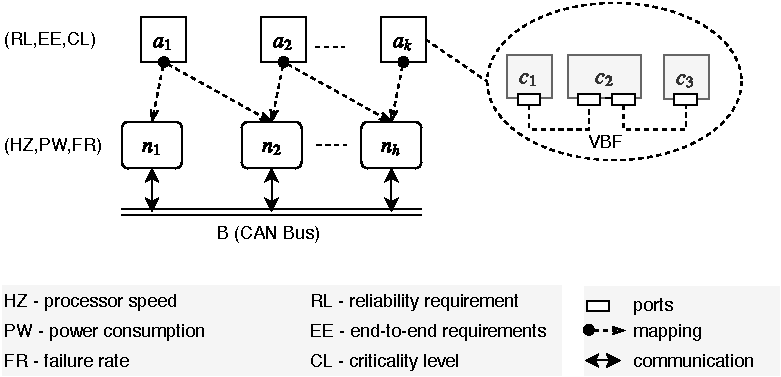
\includegraphics[scale=0.8]{system_model2}%softwareallocation
	\caption{System Model.}
	\label{fig_system}
\end{figure}
%The end-to-end timing requirements are the timing constraints over the end-to-end functional behaviors of the applications. These requirements are often specified on the \textit{cause-effect chains} consisting of software components and (potentially network messages) within the application. The reliability requirement is the expected reliability goal over a period of time $t$ in which no failure of the application experienced, and the criticality level signifies the importance of an application over other applications that have lower criticality levels, thus prioritizing the application during resource contention. The criticality levels are defined systematically, e.g., following the hazard analysis according to the ISO 26262 standard for functional safety in road vehicles~\cite{iso201126262}. 

\paragraph{Notations} For easy reading, we introduce the main notations used throught the paper as follows:

\begin{longtable}{@{}llp{0.5\textwidth}@{}}
$\bullet$ & \sexpsp{C}{c}     		             & software-component types used in \ttar\\
$\bullet$ & \sexpss{Q}{q}    		            & component replicas of type \ttsss{c}\\
$\bullet$ & \sexpss{R}[i]{r}[j]   	             & runnables of \ttsss{c}\\

$\bullet$ & \ttsexp{N}{n}         	            & computation (or computing) nodes      \\


$\bullet$ & $Power(\textbf{x})$                		& total power consumption of  $A$ in \ttx    \\
$\bullet$ & $Reliability_{a}(\x)$      					& application reliability  of $a\in A$ in \ttx              \\
$\bullet$ & $ResponseTime_{\tau}(\x)$     		& response time of  $\tau \in V(\sss{g}[k][\tau])(\x)$                       \\
$\bullet$ & $Delay_\gamma(\x)$            			& age delay of $\gamma \in \ssp{\Gamma} $   in \ttx     \\
\end{longtable}
{\footnotesize 

\subsection{Software Applications}
A software application represents an independent and self-contained user-defined software functionality, e.g., x-by-wire, electronic throttle control, flight control, etc. In AUTOSAR, software applications are developed using a \textit{Software Component} (SW-C), which is design-time concept that represents the lowest-level hierarchical element in software architecture of the software application, hence is atomic. Consequently, a software component is mapped to single computing unit. It is implented by the AUTOSAR runnables, which are schedulable pieces of codes (or objects), and contains specifications of timing behavior as well as resources requirements of the runnables. We formall represent an AUTOSAR software application as follows:

\begin{definition}[AUTOSAR Software Application]\footnote{ Note: only relevant concepts of the official AUTOSAR software application definition is assumed to avoid unnecessary complexity. }\label{def_application}
\end{definition}
\begin{figure}
	\centering
	\begin{minipage}{.475\textwidth}
		\centering
	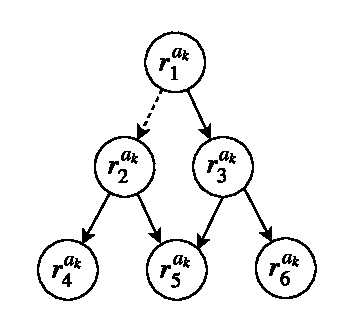
\includegraphics[width=0.7\linewidth]{img/dag_runnables}
	\caption{A Software Application Modeled as Directed Acyclic Graph.}
	\label{fig_dagcomp}
	\end{minipage}\hfill
	\begin{minipage}{0.475\textwidth}
		\centering
			\begin{tabular}{@{}llll@{}}
			\toprule
		\ttsss{c}& \ttsss{r}[k][j] &$(\mathrm{E}_h, \mathrm{P=D})$ & $\prec$ \ttsss{r} [k][i]\\ \midrule
		1&1 & $(0.1,10)$   & 2 \\ 
		2&2 & $(0.1,20)$ &  \\ 
		2&3 & $(0.1,15)$ &  \\ 
		2&4 & $(0.1,8)$   &  \\ 
		3&5 & $(0.1,12)$  &  \\ 
		3&6 & $(0.1,6)$   &  \\ 
		\bottomrule 
	\end{tabular}
		\caption{Runnables Timing Specifications.}
		\label{tbl_runnables_specs}
	\end{minipage}
\end{figure}


A path in the graph $\sss{\Gamma}=(r_i)_{i=1}^l=r_1\rightarrow,...,\rightarrow r_l$ represents a \textit{cause-effect} chain, where $r_1$ is the source of chain and $r_l$ the sink, e.g., from the appication \ttar[1]in Figure~ \ref{fig_dagcomp}, $\ssb{r}[1,1]\rightarrow \ssb{r}[2,1]\rightarrow \ssb{r}[2,3]$ is the chain, and $\ssb{r}[1,1],\ssb{r}[2,3]$, respectively are the source and the sink of the chain. A chain is a sub-functionality of the application that is triggered by a stimulus (or stimuli), e.g., pressing a brake pedal, and the corresponding response, e.g.,  vehicle braking to the desired speed level. It usually has a user-defined timing requirement, known as \textit{end-to-end} timing requirement (EE), which puts an upper-bound on the duration between the stimulus and the corresponding response of executing the chain. The set of chains in \ttar are represented as \sexpsp{\Gamma}{\Gamma}. We assume each runnable is subscribes to at least one chain.

\subsection{Scheduling Software Applications}
We assume software applications share the execution platform such as the computing units and the on-board network bus, following the mixed-criticality design~\cite{Vestal2007PreemptiveAssurance}. Thus, software applications with different software criticality should be isolated in order to prevent interference of lower-criticality applications on higher-critical applications. Assume the braking functionality of a vehicle, which is safety-criticality, is distributed over multiple computing units. Another application with infotainment functionality also shares the computing units The mixed-criticality design to this problem ensures both applications are schedulable during absence of errors, however, the braking application must also be schedulable in cases of overrun due to errors, e.g., by degrading or inhibiting the infotainment application. There are several techniques in the literature that deal with the scheduling of mixed-criticality applications on \textit{uniprocessor} systems \cite{Vestal2007PreemptiveAssurance}. In this work, we consider the \textit{partitioned criticality (PA)} (or criticality-as-priority assignment, CAPA) technique to schedule the mixed-criticality applications, which prioritizes applications based on criticality, rather than \textit{deadline} as used by the deadline monotoic assignment \cite{Baruah2011Response-timeSystems}. In contrast to other techniques, CAPA effectively counters \textit{criticality inversion}, that is unbounded blocking of higher-criticality applications by lower-criticality applications, and does not require a runtime monitoring of applications, e.g., using servers \cite{AbeniIntegratingSystems,Ashjaei2017DesigningSystems,Inam2014ThePlatforms}, albiet inefficient\footnote{Note: scheduling techniques other than the PA technique can be used with our approach to schedule the applications.}. 

The AUTOSAR software  applications are schedulable if the runnables, messages, and chains in the distributed system are schedulable, that is meet their corresponding deadlines. According to AUTOSAR~\cite{AUTOSAR2017SpecificationSoftware}, runnables are high-level schedulable objects that are mapped to tasks subsequently scheduled by AUTOSAR operating system \cite{bibid}. Thus, next, the mapping of runnables to tasks, and  schedulability of tasks and chains are explained.

\subsubsection{Runnables-to-Tasks Mapping/Transformation}\label{subsec_runnables-to-tasks}
In the mapping process, one or more runnables can be merged to optimize the runtime execution by reducing the number of schedulable tasks. Thereore, through the mappings, eventually runnable graphs are refined by task graphs as shown in Figure~{\ref{fig_appexample} (b). Moreover, the end-to-end timing analysis of chains are also defined on task chains. In this work, the following rules are applied in order to merge any runnables $a,b\in \gr{V}{\ar}$ to $v\in \gr{V}{\at}$, that is only if the following rules satisfy:
\begin{enumerate*}[label=(\roman*)]
	\item the runnables are co-hosted in the same computing unit, that is $a\mapsto n \land b\mapsto n$, where $n\in N$;
	\item activation periods of $a$ is a factor of $b$, or viceversa, and the sum of worst-case execution times of the runnables is less than the minimum of the periods.
\end{enumerate*}.
	
If the rules are satisfied, the task's timing specifications are set as follows: 
\begin{enumerate*}[label=(\roman*)]
	\item the WCET of the task is set to the sum of the WCET of the runnables, E$_h^v=$E$_h^a + $E$_h^b$, where $h:1,...,n_N$;
	\item the period and deadline of the task is set to the minimum periods of the runnables, P$_v$=D$_v=min($P$_a, $P$_b)$;
	\item otherwise, runnables are not merged, instead, each runnable that is not merged is mapped to a task while preserving the timing specifications of the runnables.
\end{enumerate*}
\begin{figure}
\vspace{0pt}\raggedbottom
	\begin{minipage}{.475\textwidth}
		\centering
		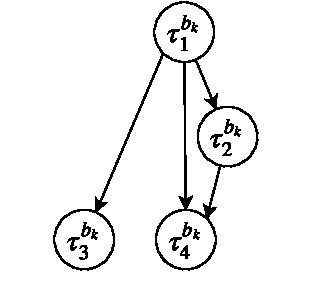
\includegraphics[width=0.6\linewidth]{img/dag_tasks}
		\caption{A Software Application Modeled as Directed Acyclic Graph.}
		\label{fig_dag_tasks}
	\end{minipage}%
\hfill
	\begin{minipage}{0.475\textwidth}
	\centering
		\begin{tabular}{@{}lll@{}}
						&&\\
			&&\\
			\toprule
			\ttsss{\tau}&$\bigcup\sss{r}[k][j]$&$(\mathrm{E}_h, \mathrm{P=D})$ \\ 
			\midrule
			1 & 1,2 &  $(0.2,10)$\\ 
			2& 3 &  $(0.1,15)$\\ 
			3& 4&  $(0.1,8)$\\ 
			4 & 5,6 &  $(0.1,6)$\\ 

			\bottomrule 
		\end{tabular}
		\caption{Tasks Timing Specifications after Merging.}
		\label{tbl_tasks_specs}
	\end{minipage}
\end{figure}

%\begin{figure}
%	\centering
%	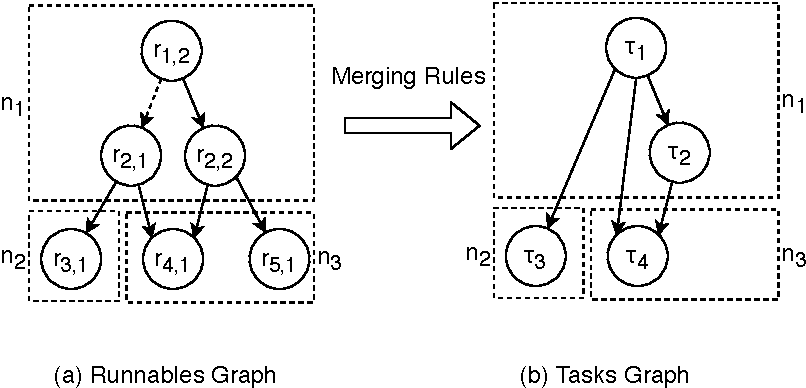
\includegraphics[width=0.7\linewidth]{img/runnable_task_dag}
%	\caption[Example of a Software Application.]{Example of a Software Application, Modeled as Directed Acyclic Graph, where $\dashrightarrow$, $\dashrightarrow$ denote triggering link, data-flow link, respectively.}
%	\label{fig_appexample}
%\end{figure}
%
%\begin{table}
%	\parbox{.45\linewidth}{
%		\centering
%		\begin{tabular}{|c|c|c|c|}
%			\hline 
%			\ttsss{r}[k][i,j] &$m_h$& $(e_h, P)$ & $\prec$ \ttsss{r} [k][i,j]\\ 
%			\hline 
%			1,1 & 1&$(1,10)$ & 2,1 \\ 
%			\hline 
%			2,1 &1& $(1,5)$ &  \\ 
%			\hline 
%			2,2 &1& $(1,15)$ &  \\ 
%			\hline 
%			3,1 & 2&$(1,20)$ &  \\ 
%			\hline 
%			4,1 & 3&$(1,10)$ &  \\ 
%			\hline 
%			5,1 & 3&$(1,20)$ &  \\ 
%			\hline 
%		\end{tabular} 
%		\caption{Runnables Timing Specifications.}
%	}
%	\hfill
%	\parbox{.45\linewidth}{
%		\centering
%		\begin{tabular}{|c|c|c|}
%			\hline 
%			\ttsss{\tau} &$\bigcup\sss{r}[k][i,j]$& $(e_h,P)$ \\ 
%			\hline 
%			1 & 1,2;2,1 &  $(2,5)$\\ 
%			\hline 
%			2& 2,2 &  $(1,15)$\\ 
%			\hline 
%			3& 3,1 &  $(1,20)$\\ 
%			\hline 
%			4 & 4,1;5,1 &  $(1,10)$\\ 
%			\hline 
%		\end{tabular} 
%		\caption{Tasks-Runnables Mappings.}
%	}
%\end{table}



\subsubsection{Scheduling Tasks and Messages}\label{subsec_response-time_analysis}
We assume tasks are scheduled using the \textit{fixed-priority preemptive scheduling polity} (FPPS)~\cite{Sha-RTS-2004}. Initally, applications are priortized based on their criticality levels followng the PA technique, and within each application the tasks are prioritized according to the \textit{deadline monotonic} (DM) priorities assignment. 
\[
cri(b_i)>cri(b_j)\implies \forall \tau_1,\in V(b_i)\forall \tau_2\in V(b_j)\ Pri(\tau_1)>Pri(\tau_2),
\]
where $\forall i,j:1,...,n_A\land i\neq j$, $cri$ and $pri$ are predicates which detemine the critiality and priority of tasks $\tau_1,\tau_2$, respectively; $V(b_i), V(b_j)$ are returns the tasks nodes, respectively for $b_i$ and $a_j$.

The schedulability of tasks is checked by the classical response-time analysis shown in Equation (\ref{eqn_responsetimeanalysis}) \cite{Baruah2011Response-timeSystems,Baruah2011Response-timeSystems}, which computes the worst-case response time of each task, denoted by $delta_\tau$. According to the analysis, if the response time of each task is less than or equal to its deadline, that is $\delta_\tau\leq Deadline_\tau$, the taskset is schedulable otherwise it is not. 

\begin{align}
\label{eqn_responsetimeanalysis}
R_\tau=C_\tau+\sum_{j\in h\!p(\tau)}
{
	\ceil[\Big]
	{
		\frac{R_\tau}{P_j}
	}C_j
},
\end{align}
where $C_\tau,C_j$ are exection times of the lower and higher tasks, respectivel; $h\!p(\tau)$ is the predicate that returns the higher-priority tasks of task $c_\tau$.

%In this work, we assume heterogeneous computating nodes, therefore the schedule that delivers lower power-consumption of a node is considered the effective and efficient. The power-consumption of a node is computed linearly from the utilization of a taskset mapped to a specific node as well as from its power-specification parameters, and is discussed in detail in Subsection \ref{sec_problem}.

The messages in the CAN bus are scheduled using a fixed, non-preemptive scheduling policy. Similar to the tasks, the priority of messages followes the PA techniques to achieve the mixed-criticality requirement. This can easily be achived by inheriting the priority of sender task, that is $pri(m)=pri(\tau)|\tau = pre(m)$, where $pre(m)$ finds the sender task. The schdulability of messages is checked using the classical response-time analysis of the CAN network, presented by Rob Davis et. al~\cite{RobDavis-CAN-2007} as shown in Equation~(\ref{eqn_responsetimeanalysisCAN}). Thus, the worst-case response time of a message is computed as the summation of its \textit{jitter} time (that is, the time  taken by the sender task to queue for transmittion) $J_m$, the \textit{interferance} time (that is, the message delay in the queue) $w_m$, and its \textit{transmission} time  (that is, the longest time for a signal or data to be transmitted) $c_m$.
\begin{align}
\label{eqn_responsetimeanalysisCAN}
R_m&=J_m+w_m+c_m\\
\label{eqn_interference}
w_m&=B_m+
\sum_{\forall k\in hp(m)}
{
	\ceil[\Big]
	{
		\frac{w_m+\tau_{bit}}{P_k}
	}c_k
}\\
\label{eqn_iblocking}
B_m&=\max_{\forall k\in lp(m)}(c_k),
\end{align}

Note: we assume no jitter, therefore, the interferenece formula is reduced as shown in Equation (\ref{eqn_interference}), where $B_m$ is the blocking time caused by the lower-priority messages using the CAN bus (since it is non-preemptive) and is computed by Equation (\ref{eqn_iblocking}); $hp(m)$ finds the higher-priority messages, which delay the trasmission of the message $m$ in the queue as well as in the transmission.

\subsubsection{Scheduling Cause-effect Chains}\label{subsec_cause-effect_chains}
Due to the independently clocked tasks, scheduling the chains on the execution platform is not trivial. It results in undersampling effects when a frequently executing task communicates with a less frequently task. In the opposite case, it results in oversampling effects. Thus, a signal propagating across a chain that consists of independently clocked tasks of different periods normally encounters multiple paths due to the various effects. The different paths are defined over activation of tasks instances in the chain, and usually have different latencies (or delay semantics), which are discussed in detail by Mubeen et al.~\cite{mubeen2013support} in the context of single-register buffer communication,  which is a common practice in control systems design, e.g., automotive software applications~\cite{Becker2017End-to-endSystems}. In this work, we demonstrate the two widely used semantics in the automotive domain: \textit{age} delay and \textit{reaction} dealy. Consider the chain $\sss{\tau}[k][1][b]\rightarrow \sss{\tau}[k][2][b]\rightarrow \sss{\tau}[k][4][b]$ of the task graph \ttat[1] from Figure~\ref{fig_dag_runnables}. Assume the chain is mapped on the computing units $n_1$ and $n_2$ as illustrated in Figure~\ref{fig_cause_effect_chain}, and communicate using the single-register buffers.
\begin{figure}
	\centering
	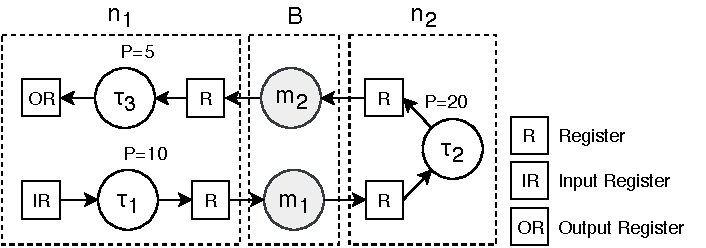
\includegraphics[width=0.7\linewidth]{img/cause_effect_chain_ntk}
	\caption{A Cause-effect Chain, mapped on nodes $n_1$ and $n_2$.}
	\label{fig_cause_effect_chain}
\end{figure}

The tasks $\tau_1$ and $\tau_2$ execute on node $n_1$, whereas task $\tau_3$ executes on node $n_2$. The execution time line of the chain over two hyper-periods are illustrated in Figure~\ref{fig_timedchainntk}. Note: $\tau_2$ communicates with $\tau_3$ via a CAN bus, which is not shown in the figure for simplicity. The red inverted arrows in the figure represent the reading of data from the input register, whereas the dashed-curve arrows represent the timed paths through which the data propagates from the input to the output of the chain. Thus, the age delay is the time elapsed between a stimulus arriving a the input register and its corresponding latest non-overwritten response at the output register, that is between the $3^{rd}$ instance of  $\tau_1$  and the $10^{th}$ instance of $\tau_3$. It is frequently used in the control systems applications where freshness of data is paramount, e.g., braking a car over a bounded time. And, the reaction delay is the earliest time the system takes to respond to a stimulus that ``just missed" the read access at the input of the chain. Assume that data arrives just after the start of the $1^{st}$ instance of $\tau_1$ execution. The data corresponding to this event is not read by the current instance of $\tau_1$. In fact, the data will be read by the $2^{nd}$ instance of $\tau_1$. The earliest effect of this data at the output of the chain will appear at the $7^{th}$ instance of $\tau_3$, which represents the reaction delay. This delay is useful in the body-electronics domain where first reaction to events is important, e.g., in the button-to-reaction applications. For detailed discussion of the different delay semantics, we direct the reader to check research work by Mubeen et al.~\cite{mubeen2013support}. 
\begin{figure}
	\centering
	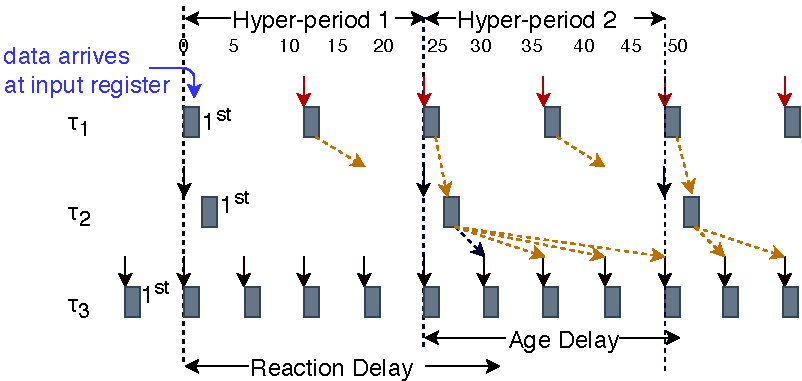
\includegraphics[width=0.9\linewidth]{img/timedchain_ntk}
	\caption{Reaction and Age Delays of the Cause-effect Chain, Shown in Figure {\ref{fig_causeeffectchainntk}}.}
	\label{fig_timedchainntk}
\end{figure}

The age delay is computed using Equation (\ref{eqn_agedelay_singlenode}) and Equation (\ref{eqn_agedelay_multinode}) for a single node and multiple nodes, respectively.

\begin{align}
	\label{eqn_agedelay_singlenode}
	\Delta^{sub}(\Gamma) &= \alpha(sink(\Gamma))-\alpha(source(\Gamma)) + \delta(sink(\Gamma)) & \text{single unit}\\
	\label{eqn_agedelay_multinode}
	\Delta(\Gamma)&=\sum_{i\in I_{\Gamma}}{\Delta^{sub}(i)} + \sum_{j\in  J_{\Gamma}}{\delta^{msg}(j)}, &\text{muliple units}
\end{align}
where $\alpha(\tau)$ computes the activation of the task $\tau$, based on the age-delay semanics.

Assume $\Gamma \in \ssp{\Gamma}$ is a chain, if the chain is mapped on a single computing unit, the age delay is a mere difference between the activation of the sink task $\ssb{\alpha}[\tau_j]$ and the activation of the source task $\ssb{\alpha}[\tau_i]$ plus the worst-case response time of the sink task $\ssb{\delta}[\tau_j]$ in the longest timed path according to the semantics of the age delay. On the other hand, if the chain is mapped to multiple nodes, the age delay $\Delta_{multi}$ can be compositionally computed~\cite{Feiertag2009ASemantics} as follows: the chain is partitioned  into a set of sub-chains per node, indicated by the predicate $subch(\Gamma)$, and for each sub-chain $a\in subch(\Gamma)$, the age delay is computed recursively using the same method to used to compute the age delay for a single node, and the result is added to the response-times of the messages involved in the chain, $msg(\Gamma)$.

\subsection{Reliability of Software Applications}\label{sub_reliability}
In this context, \textit{software application reliability} refers to the probability that a software application functions correctly by the time $t$, or within the time interval $[0, t]$ \cite{Goel1985SoftwareApplicability}. Redundancy is the most common way for implementing fault tolerance and increasing the reliability of a system. Redundancy can be implemented according to different schemes, such as hot stand-by, cold stand-by, etc.~\cite{Dubrova2013Fault-tolerantDesign}, which differ on the number of replicas that are active as well as the methods for detection and compensation of faulty replicas. In our system model, we consider the hot-standby scheme, where replicated components maintain the same state, but only one replica (the so-called \textit{primary}) effectively acts on the environment, for instance issuing an input. The primary software component will be denoted as \ttsss{q}[k][i,1], whereas the secondary software component, which is in the stand-by, by \ttsss{q}[k][i,2], etc., for a software application $A_k$.

%Note: the software components are replicated unless the reliability requirements of applications are satisfied.


In this work the details of the redundancy scheme are abstracted away under the following assumptions:
\begin{enumerate*}[label=(\roman*)]
    \item Software does not contain design errors. This has two implications: first, that hardware elements, i.e. computing nodes and communication buses, are the only causes of failure and, second, that introduction of N-version programming is not required. Different replicas of the same software component execute exactly the same program.
	\item Hot stand-by redundancy (also known as Primary/backup) is used for detection and replacement of failed components.
	\item Software components need to be replicated only if the application's reliability requirement is not met without replication, otherwise they are not replicated.
	\item The time needed to detect and replace a faulty component is considered negligible and will not be taken into account in the response time analysis of tasks and delay calculation of cause-effect chains;
	\item Because of its simplicity, the mechanism for detection and replacement of faulty components will be considered fault-free, and therefore will not be included in the reliability calculations
\end{enumerate*}

Note that under these assumptions, the reliability of a software application is equivalent to the reliability of the platform on which it is deployed. The reliability of a computing unit (and of the bus) can be easily calculated as $e^{\lambda t}$, where $\lambda$ is an exponentially distributed failure-rate. However, calculating the reliability of the whole execution platform is not trivial for the case with replication. In particular, the traditional series-parallel reliability approach cannot be applied because of the \textit{functional} interdependencies created between computing nodes as the result of replication and allocation. To illustrate the difficulty, let us assume a software application $A_k$, having  component configurations with and without replication as shown Table \ref{fig_depwr} and \ref{fig_depwor}, respectively, where $\sss{q}[k][i,j]$ is the $j^{th}$ software-component replica of software-component type $\sss{c}\in \sss{C}$. Note: for readability of the example, we remove the superscript $k$.
\begin{figure}
	\begin{subfigure}{.5\textwidth}
		\centering
		\begin{tabular}{ccc}
			$n_1$ & $n_2$ & $n_3$\\
			\hline
			\ttssb{q}[1,1]&\ttssb{q}[2,1]& \\
			\ttssb{q}[3,1]& & \\
			\hline
		\end{tabular}	
		\caption{Without Replication.}
		\label{fig_depwor}
	\end{subfigure}%
	\begin{subfigure}{.5\textwidth}
		\centering
		\begin{tabular}{ccc}
			$n_1$ & $n_2$ & $n_3$\\
			\hline
			\ttssb{q}[1,1]&\ttssb{q}[2,1]& \ttssb{q}[2,2]\\
			\ttssb{q}[3,1]& \ttssb{q}[1,2]& \ttssb{q}[3,2]\\
			\hline
		\end{tabular}
		\caption{With Replication.}
		\label{fig_depwr}
	\end{subfigure}%
	\caption{Partition of the Software Application $a_1$.}
	\label{fig_deployment}
\end{figure}

The reliability of the software application without replication forms a series path, indicated by the reliability block diagram (RBD) of Figure~\ref{fig_rbd}a, hence is computed as products of the reliability of $n_1,n_2$ and $B$. However, with replication, two computing nodes can form as series and parallel to service the software application,  e.g., due to \ttssb{q}[1,1] and \ttssb{q}[2,2] or \ttssb{q}[3,2], $n_1$ and $n_3$ make series, and due to \ttssb{q}[3,1] and \ttssb{q}[3,2], the nodes make parallel, to realize a partial functionality of the application. In this case, the series-parallel diagram depicted in Figure~\ref{fig_rbd}b does not accurately capture the reliability calculation of the application with replication. Note: the red-dashed line between $n_1$ and $n_3$ indicates the possibility of the computing nodes becoming series. To overcome this problem, we will use an exact technique for reliability calculation based on the enumeration of the different failure states of the computing nodes; that is, the different failure states of the execution platform are enumerated exhaustively, and subsequently, the total probability the software application functions is computed. This technique will be discussed in great length in Subsection~\ref{subsec_reliability_constraint}.
\begin{figure}
	\centering
	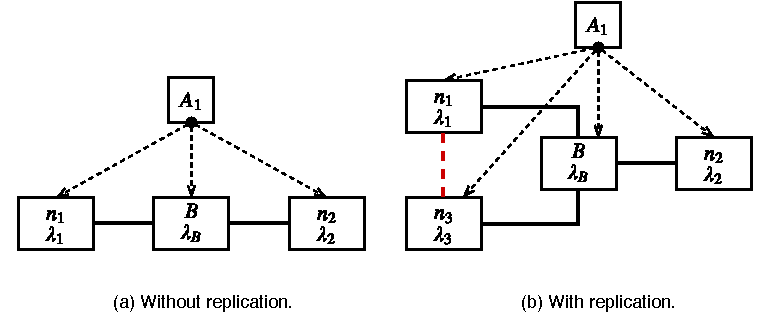
\includegraphics[width=0.8\linewidth]{img/rbd_replication}
	\caption{Reliability Block Diagrams of the Software Application.}
	\label{fig_rbd}
\end{figure}




\section{Problem Model}\label{sec_extrafunc}
The software allocation problem is a type of job shop scheduling with constraints, as such it is a discrete optimization problem \cite{}. The solution to the allocation problem is represented by a vectormatrix $\x=\{\xsp{k}:k=1,...,N_a\}$, where \ttxsp{k} is a matrix of size $N_c\times K$, and \ttssx{x}{k}{ij}$=k\in \{1,…,N_m\}$ represents the mapping of the software component replica \ttssx{c}{k}{ij} to the computation node $m_k$.
\begin{equation}
\label{fig_pso_solution_representation}
\bspx{k}=
\begin{bmatrix} 
\ssx{k}{11} & \ssx{k}{12} & \dots & \ssx{k}{1K}\\
\ssx{k}{21} & \ssx{k}{22} & \dots & \ssx{k}{2K}\\
\vdots & \vdots & \ddots & \vdots\\
\ssx{k}{N_c1} & \ssx{k}{N_c2} & \cdots & \ssx{k}{N_cK}
\end{bmatrix}
\end{equation}

In this work, the main objective of the allocation problem is to satisfy the user-defined requirements, namely reliability requirements, end-to-end timing requirements, and criticality of the software applications $A_i$ by effectively mapping the software components to the computation nodes, $C^{(k)}\mapsto M$. Furthermore, the components are allocated efficiently to minimize the total power consumption $Power(\textbf{x})=\sum_{m\in M'}{P_{m}(\textbf{x})}$ of the applications by selecting lower-power consuming nodes $M'\subseteq M$, provided the requirements are met, where $P_{m}(\textbf{x})$ is the power consumption of node $m$ on the mapping $\textbf{x}$. Power consumption, in this context, refers to the energy usage of electronic components in the integrated circuits of the node, e.g., processor, memory, I/O devices, etc., per time unit. 

%Power consumption refers to the energy usage of electronic components in an integrated circuit, e.g., processor, memory, I/O devices, etc., per time unit. 
There are several power consumption models and different techniques to estimate the power consumption of a computing node. In this work, we employ a technique based on processor load (or \textit{Processor Utilization}) to estimate the average power consumption of a computation node. Specifically, we use the linear polynomial model proposed by Fan et al. \cite{Fan2007PowerComputer}, which is shown in (\ref{eqn_powerconsumption}). The model states that the power consumption of a node is directly proportional to its load, and is inductively formulated from experimental results:
\begin{equation}
\label{eqn_powerconsumption}
f_p(u)=P_{idle} + (P_{busy}-P_{idle})*u,
\end{equation}

where $u$ is the utilization (or load) of a computation node, $p_{idle}$ and $p_{busy}$, respectively, refer to the power consumption of a node measured at minimum and maximum processor loads. Such measurements can be obtained by running performance benchmark suits, e.g., MiBench \cite{Guthaus2001MiBench:Suite}, AutoBench \cite{EMBC2018AutoBenchProcessors}, etc., which is computed based on the utilization of the node via the linear power consumption model shown in Equation (\ref{eqn_powerconsumption}).

Consequently, the power consumption of a node $m$ for a given mapping $\textbf{x}$ is computed using Equations (\ref{eqn_powerconsumption_x}-\ref{eqn_util_component}), by calculating first the node's utilization $U_m(\textbf{x})$ using Equation (\ref{eqn_util_x}). The node's utilization is computed from the set of components allocated to it (which are $\forall_{ij} x_{ij}=m$) using Equation (\ref{eqn_util_x}). And the utilization of a component on the node $m$ is computed from its constituent tasks $T_c$ using Equation (\ref{eqn_util_component}).
\begin{align}
	\label{eqn_powerconsumption_x}
nodPow(\textbf{x}) & =f_p(nodUti(\textbf{x},m))                         &  \\
	\label{eqn_util_x}
nodUtil(\textbf{x},m)           & = \sum_{k}{\sum_{i}{\sum_{j}{comUtil(m,c)}}}|\xkij=m         & \text{, where } c=\sss{C}\\
	\label{eqn_util_component}
comUtil(m,c)              & = \sum_{r\in c.R} \frac{r.e_m}{r.\tau.P}, &
\end{align}

where $c.R$ is set of runnables in component $c$, $r.e_m$ and $r.\tau.P$ are the execution of runnable $r$ on node $m$ and its period, respectively.

The applications requirements are modeled as constraints that need to be satisfied in the allocation problem. The constraints formulations are shown in the following subsections, respectively for reliability, timing and other design constraints such as related to runnables-to-tasks merging and replication.

\subsection{Software Application Reliability Constraints}\label{subsec_reliability_constraint}
The applications reliability constraints ensure the mapping $\textbf{x}$ satisfies the user-defined reliability requirements, that is $ \forall k\in [1,n_A]\ \rel_{A_k}(\xsp{k})\leq RelReq_{A_k}$. 
The reliability  is computed from the execution framework that is provided to run the application, which consists of computation nodes \ttssp{M} and the shared CAN bus B, as shown in Equation (\ref{eqn_appreliability_app}). The nodes \ttssp{M} host the components \ttssp{C} and are determined by searching the mapping \ttxsp{k}  in polynomial time using Equation (\ref{eqn_nodes_app}).
\begin{align}
	\label{eqn_appreliability_app}
	&Reliability_{A_i}(\x)=Reliability_{A_i}(\ssp{M})*Reliability(B)\\
	\label{eqn_nodes_app}
	&\ssp{M}=\{e|e\in M \land \forall ij (e=m_h) \},\mbox{ where } h=\ssx{k}{ij} 
\end{align}

The reliability of the nodes, $Reliability_{A_i}(\ssp{M})$ with respect to the application ${A_k}$ is calculated using the \textit{state-enumeration} technique \cite{Lucet1999ExactReliability}  as shown in Equations (\ref{eqn_appreliability}). According to the technique, the reliability is basically the total probability that the application $A_k$ \textit{functions} under mutually exclusive and uniformly distributed failure-events of the nodes, represented by $\ssp{\mathcal{F}}(\ssp{M})=\{\textbf{0},\textbf{1}\}^{\ssp{M}}$, where  \textbf{0} means node fails, \textbf{1} means  node is operational. An event $\omega\in \mathcal{F}_{A_k}(\ssp{M})$ represents the states of nodes by a sequence of 0-1 variables $(b_1,...,b_n)$, where $\omega.b_i$ denote the state of node $m_i\in \ssp{M}$. %as the state of the nodes $\ssp{M}=\{e_1,...,e_n\}$ by $s\in \ssp{\mathcal{F}}(\ssp{M})=(b_{e_1},...,b_{e_n})$, where $n=|\ssp{M}|$, whereas the state of a node is referenced by $s.b_{e}$.
\begin{align}
\label{eqn_appreliability}
Reliability_{A_i}(\ssp{M})&=\sum_{s\in \ssp{\mathcal{F}}|g(A_i, s)=1}probability(s)
\end{align}

The fact that an application functions $g(A_k, s)$ is defined via its inverse, which is \textit{software application failure}, deductively as follows:
\begin{definition}[Software Application Failure]
The application $A_k$ fails in the event $\omega \in \ssp{\mathcal{F}}(\ssp{M})$ if there exists a component type \ttsss{c} where all of its replica \ttsss{Q} \textit{fail}, otherwise, the application functions, as shown in Equation (\ref{eqn_app_failure}).  A component replica $\sss{q}[k][ij]\in \sss{Q}$ fails if the node that host it $m_h$ fails, where $h=\xkij$.  
\begin{align}
\label{eqn_app_failure}
g(a, \omega)&= 
\begin{cases}
\textbf{0} & \mbox{ if } \exists i\forall j\ (m_h\in \sss{M}[k][\omega] )\\
\textbf{1} & \mbox{ otherwise }
\end{cases}\\
\label{eqn_appreliability_node_s}
\sss{M}[A_k][\omega]&=\{e|e\in \ssp{M} \land (\omega.b_e=1) \},
\end{align}
\end{definition}
where \ttsss{M}[k][\omega] denote the nodes that function at the event $\omega$, and can be found by searching the nodes \ttssp{M} with state $\omega.b_e=1$ in constant time , as show in Equation (\ref{eqn_pro}).

The probability that a nodes-failure event $\omega$ occurs is computed as a product of the probabilities of its consitutuent elements $\omega.b$ as shown in Equation (\ref{label}).
\begin{equation}
\label{eqn_pro}
	\prod_{(m,b)\in (M,\omega)}{\lambda_m*(1-b)+(1-\lambda_m)*b}
\end{equation}
where $\lambda_m$ is the failure-rate of node $m$.

\subsection{Timing constraints}
The timing constraints ensure that the applications are schedulable on the execution platform, that is the tasks and cause-effect chains of each application meet their deadlines. The schedulability of each task is checked using the worst-case response-time anlaysis presented in Subsection \ref{subsec_responsetimeanalysis}, and for the cause-effect chains using delay analysis shown in Subsection \ref{subsec_causeeffectchains}. Before we formulate the timing constraints, first we derive the task graph for a mapping \ttx from the runnables graph \ttsss{g}[k][r], that is using Equation (\ref{eqn_generatetasksgraphs}).  Using Equation (\ref{eqn_uprdaterunnables}), we update the runnables with nodes information, to which they are mapped by traversing elements of the mapping \ttx, $\xkij$, in linear-time complexity $O(n)$, where $n=|\x|*N_r$, and $N_r$ is the total number of runnables in the system. Consequently, we traverse the runnables graphs, and apply the merging rules stated in the Subsection \ref{subsec_autosarsystem} to derive the tasks graphs. In the case that only runnables from the same component are mapped to at least on task, the derivation of tasks graphs is indpedent of the mapping \ttx, and thus can be performed before the mapping activity. However, the tasks graphs has to be updated with the nodes information after the mapping \ttx is identified.
\begin{align}
\label{eqn_uprdaterunnables}
&\forall k,ij\ \forall r\in \sss{H}[k][i,j]\ r.node = n_h& \mbox{, where } h=\xkij\\
\label{eqn_generatetasksgraphs}
&\forall k\ \sss{g}[k][r](\x)\xrightarrow{\text{Eqn. (13);Merging Rules}}\sss{g}[k][\tau](\x)
\end{align}

where $\sss{H}[k][i,j]$ is the set if runnables that implement component $\sss{q}[k][i,j]$.

%To calculate the delay, the response time of tasks is a prerequisite, therefore, the latter is calculated first as follows.

\subsection{Tasks Timing constraints}
The tasks timing constraints states that the worst-case response time of each task in the system meets its respective deadlines for a mapping \ttx, that is $\forall k\forall \tau\in V(g_r(\x))$ $ResponseTime(\tau)\leq Deadline(\tau)$, where $V(\sss{g_r(\x)})$ is the nodes in the tasks graphs. To compute the worst-case response time of the tasks, first we partition the tasks per node, that is tasks mapped to the same node grouped, represented by the $\ssb{T}[n_h]$, by traversing the tasks graphs using Equation (\ref{eqn_tasks_nodes}). The complexity of this equation, considering an adjucency matrix tasks graphs representation is linear-time $O(N_a*n^k)$, where $n$ is the sum of the order and size of graph $\sss{g}[k][\tau](\x)$.
\begin{align}
\label{eqn_tasks_nodes}
T_{m_h}&=\{e | e\in V(\sss{g}[k][\tau](\x)) \land e.node == m_h, \}& \mbox{ for all } h=1,...,n_N
\end{align}

Then, we calculate the response time of each task $\tau \in T_{m_h}$ by invoking the response-time analyais formula and construct the tasks timing constraints as shown in Equation (\ref{eqn_tasks_constraints}).
\begin{align}
\label{eqn_tasks_constraints}
\forall \tau\in T_{m_h} \delta(\tau,m_h)&\leq Deadline(\tau)& \mbox{ for all } h=1,...,\n{M}\\
\end{align}

\subsection{Cause-effect Chains Timing constraints}
For a mapping \x, the age delays of cause-effect chains should meet thier respective end-to-end requirements, that is $\forall k\forall ij\ AgeDelay_\Gamma(\x)\leq \sss{E2eReq}[k][\Gamma]$, where $\Gamma\in \sss{\Gamma}$. To calculate the age delays, first we identify the messages scheduled by the CAN bus for the mapping \ttx using Equation (\ref{eqn_messages}). 
\begin{align}
\label{eqn_messages}
	M=\{e|\forall (a,b)\in g_\tau(\x)\forall n\in N\ (a\mapsto n \land b\mapsto n=false)\implies createMsg(e)\},
\end{align}
where $Period(e)=Period(a)$, that is the message inherits the period of its predecessor (or sender) task. Accordingly, we update only the chains that communicate over the shared CAN bus to incorporate the messages, that is $\sss{\Gamma}=\{\sss{\Gamma}[k][1],e^*,\sss{\Gamma}[k][N]\}$, where $e\in V(g_\tau(\x))\cup M$. Using Equation (\ref{eqn_agedelay}), we calculate the age delays of each cause-effect chains. 



\subsection{Software Allocation Optimization Problem	}\label{sec_allocation}
In this section, we define the allocation problem of a fault-tolerant software application on a network of heterogeneous nodes which is formulatd as ann optimization problem as shown in Equation (\ref{eqn_const_func}). The optimization problem considers minimizing of power consumption $p(x)$ as the objective while fulfilling timing (\ref{eqn_timing}) and application reliability requirements (\ref{eqn_reliability}) of the software applications as well as satisfying design and hardware constraints, e.g., respecting affinity of software components to dedicated nodes.
\begin{align}
\label{eqn_optimization}
\min_{x\in X}\;\;& P(\textbf{x}) & \\
\text{Subj to:} &\\
& ResponseTime_i(\textbf{x}) \leq Deadline_i & \text{for }\tau_i\in T, i=1,2,...,N_\tau \\ 
\label{eqn_e2e}
&Delay_i(\textbf{x}) \leq EndToEnd_i & \text{for }\Gamma_i\in \Gamma, i=1,2,...,N_\Gamma \\
\label{eqn_reliability}
&Reliability_i(\textbf{x}) \leq RelReq_i & \text{for }a_i\in A, i=1,2,...,N_A\\
\label{eqn_mapping}
&StaticMapping_i(\textbf{x})\models \top & \text{for }c_i\in C, i=1,2,...,N_c
\end{align}
where $x\in X$ is a feasible solution from the search space
$X$, is the search space of the problem,  are a set of timing specification constraints, $Timing\in \Bbb R^n$ is a set of timing boundaries, and $c^{reliability}\in \Bbb R^n$ is a set of reliability boundaries.

In the rest of this section, we show the ILP model and the PSO algorithm of the software allocation problem, which are validated on an automotive use case and evaluated for performance in the next section. Throughout this section, we use a simple running example of a system model in order to demonstrate our proposed ILP model and the PSO optimization algorithm.

\subsection{Running Example}
The example employs an AUTOSAR system, which consists of a software application model and a hardware platform model, as well as functional and extra-functional requirements such as timing and reliability of the software application. The software application is modeled as a digraph of runnables, which is shown in Figure \ref{fig_application}. It consist of 50 runnables, 35 cause-effect chains (or paths), with their activation patterns and timing specifications shown in Table \ref{tbl_requirements}. The timing specifications of the runnables as well as the software components from which the runnables are instantiated are shown in Table \ref{tbl_comps_config}. The hardware platform model consists of three computation nodes, with specifications shown in Table \ref{tbl_nodes_specification}.
\begin{figure}[t!]
\centering
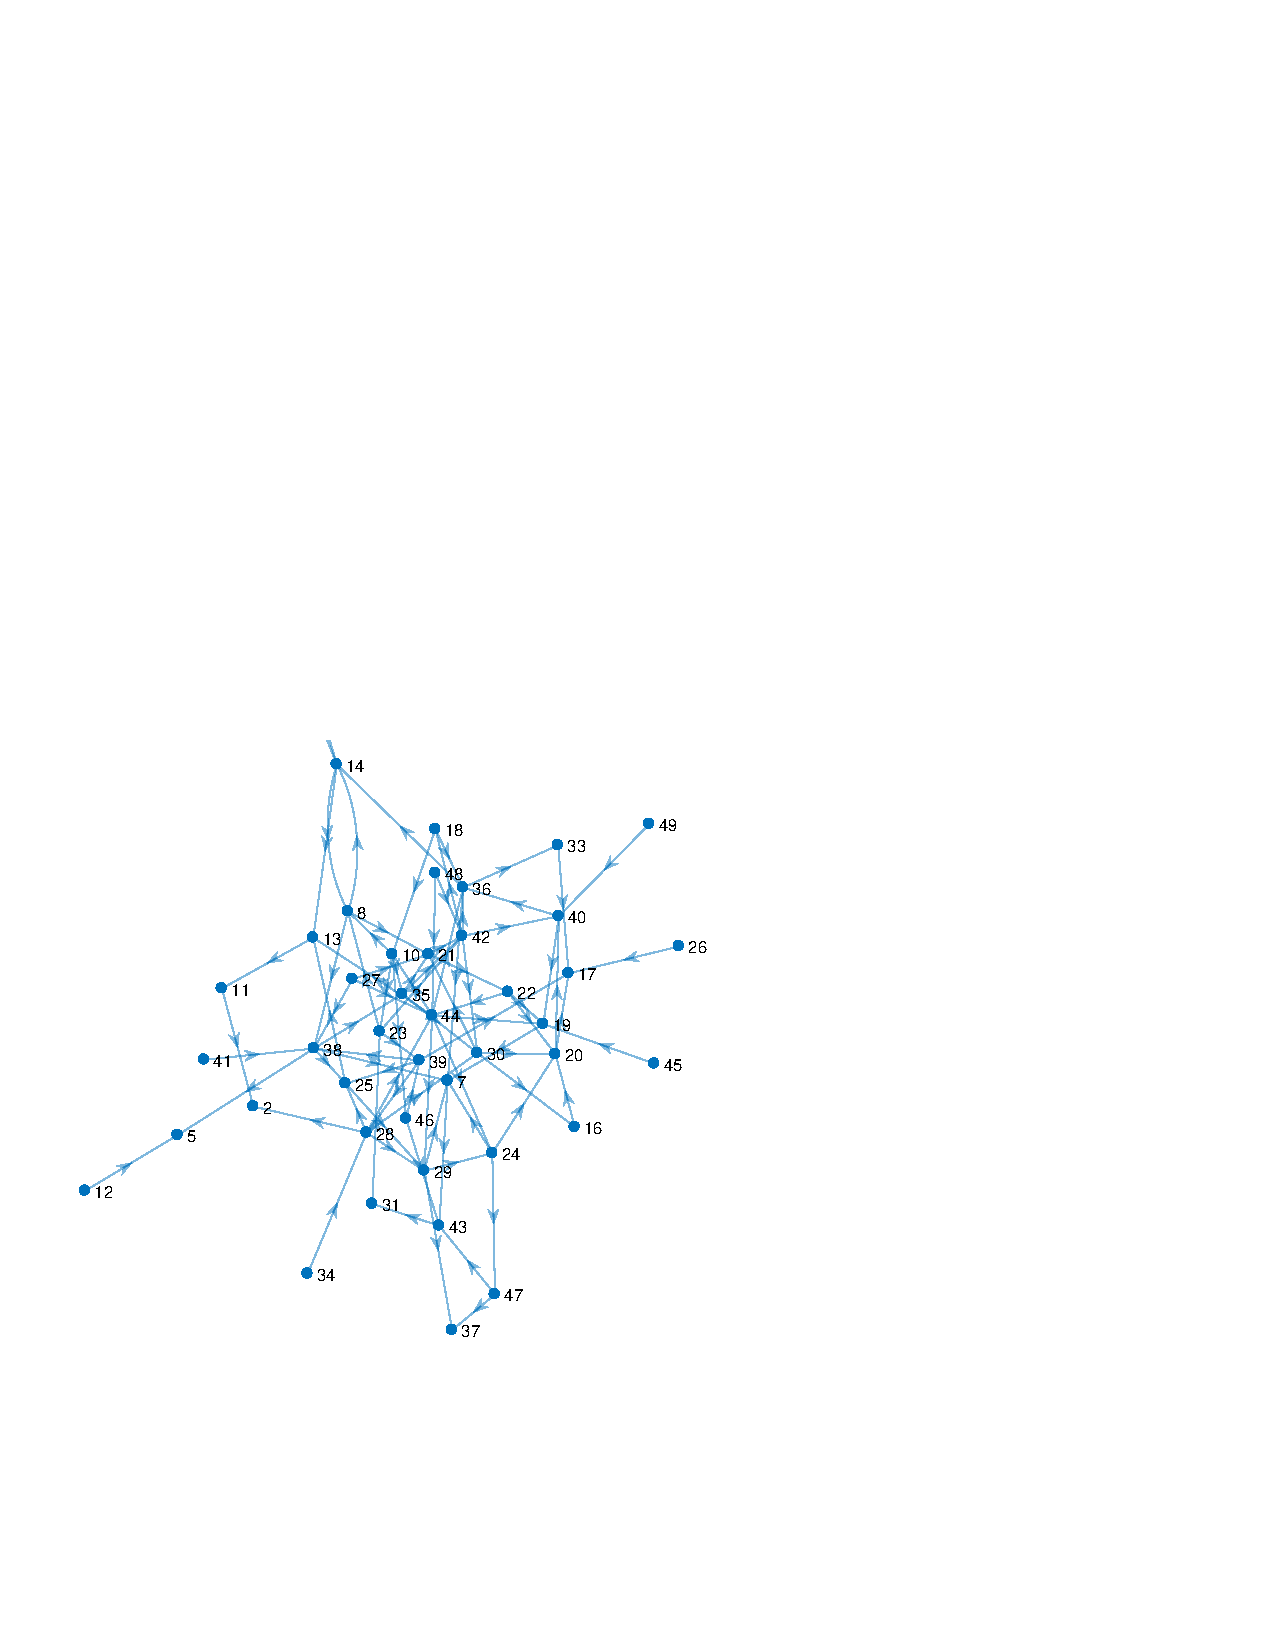
\includegraphics[width=0.8\linewidth]{dag}
\caption{A Directed Acyclic Graph of the Running AUTOSAR Software Application, Runnables = 50, Paths = 35, Activation Patterns shown in Table \ref{tbl_requirements}.}
\label{fig_application}
\end{figure}
\begin{center}
\small
\begin{minipage}{.5\textwidth}%
\centering
\begin{tabular}{@{}p{0.25cm}lll@{}}
\toprule
C& $r_i$ & $(e_{r_im_1}, e_{r_im_2}, e_{r_im_3})$ & $period$\\ \midrule
\multirow{4}{4em}{c1} 
&$r_1$ & (0.030, 0.060, 0.090) & 1\\
&$r_2$ & (0.041, 0.081, 0.122) & 2\\
&$r_3$ & (0.083, 0.167, 0.250)  & 5\\ 
&$r_4$ & (0.310, 0.620, 0.930) & 10 \\[0.3em]
\hline
\multirow{2}{4em}{c2} 
&$r_1$ & (0.310, 0.620, 0.930) & 10\\
&$r_2$ & (0.310, 0.620, 0.930) & 10\\
&$r_3$ & (0.310, 0.620, 0.930)  & 10\\ 
&$r_4$ & (0.310, 0.620, 0.930) & 10 \\[0.3em]
\hline
\multirow{2}{4em}{c3} 
&$r_1$ & (0.310, 0.620, 0.930) & 10\\
&$r_2$ & (0.291, 0.583, 0.874)) & 10\\
&$r_3$ & (0.291, 0.583, 0.874)  & 20\\ 
&$r_4$ & (0.291, 0.583, 0.874) & 20 \\[0.3em]
\hline
\multirow{2}{4em}{c4} 
&$r_1$ & (0.291, 0.583, 0.874) & 20\\
&$r_2$ & (0.291, 0.583, 0.874)) & 10\\
&$r_3$ & (0.291, 0.583, 0.874)  & 20\\ 
&$r_4$ & (0.093, 0.186, 0.279) & 50 \\[0.3em]
\hline
\multirow{2}{4em}{c5} 
&$r_1$ & (0.420, 0.841, 1.261) & 100\\
&$r_2$ & (0.420, 0.841, 1.261)) & 100\\
&$r_3$ & (0.420, 0.841, 1.261)  & 100\\ 
&$r_4$ & (0.420, 0.841, 1.261) & 100 \\[0.3em]
\bottomrule
\end{tabular}
\captionof{table}{Specification of Components.}
\label{tbl_comps_config}
\end{minipage}~
\begin{minipage}{.45\textwidth}
\begin{center}
    \begin{tabular}{@{}lll@{}}
    \toprule
    Activation, $AP$ & Share & Time, ms \\ \midrule
    $\tau_1$ & 50  & 50\\
    $\tau_1\rightarrow\tau_2$ & 20  & 100\\
    $\tau_1\rightarrow\tau_2\rightarrow\tau_3$ & 20  & 200\\
    $\tau_1\rightarrow\tau_2\rightarrow\tau_3\rightarrow\tau_4$ & 10  & 400\\
    \bottomrule
    \end{tabular}
    \captionof{table}{Activation Patters of Cause-effect Chains, their Share and End-to-end Timing Requirements.}
    \label{tbl_requirements}
\end{center}
\begin{center}
    \begin{tabular}{@{}llll@{}}
    \toprule
    M  & $P_{idle}$& $P_{busy}$& $\lambda$ \\ \midrule
    $m_1$ & 50.0& 140.0 &1.0E-3  \\
    $m_2$ & 10.0& 100.0 &1.0E-4  \\
    $m_3$ & 10.0& 140.0 &1 .0E-5 \\ \bottomrule
    \end{tabular}
    \captionof{table}{Computation Nodes Specification.}
    \label{tbl_nodes_specification}
\end{center}
\end{minipage}
\end{center}

In the next subsequent subsections, we propose a metaheuristic approach which is based on Particle Swarm Optimization (PSO) and hybrid PSO. Furthermore, we elaborate the approach using the presented running example.

\section{Software Allocation Problem}\label{sec_allocation}
In this section, we show our ILP model and the software-to-hardware allocation of a fault-tolerant application on heterogeneous nodes. Equation (\ref{eqn_const_func}) defines the objective function for power consumption, with constraints on timing (\ref{lbl_deadline_constraint}) (\ref{lbl_e2e_constraint}) and application reliability (\ref{lbl_reliability_constraint}). 
\begin{align}
\label{eqn_const_func}
\min_{x\in X} P(x) \\
\text{Subjected to:}\nonumber\\
\label{lbl_deadline_constraint} 
ResponseTime(x) \leq \mathrm{Deadline}\\ 
\label{lbl_e2e_constraint}
Delay(x) \leq \mathrm{E2eReq} \\
\label{lbl_reliability_constraint}
Reliability(x) \leq \mathrm{RelReq}
\end{align}

The timing constraints consist of meeting the individual tasks deadlines $Deadline$  as well as the end-to-end timing requirements of cause-effect chains $\mathrm{E2eReq}$ (\ref{lbl_e2e_constraint}) in the distributed system. The reliability constraint ensures that a feasible solution meets the application reliability requirement $\mathrm{RelReq}$. The decision variable $x$ is a 3-dimensional binary matrix that represents a feasible solution, where $x^k_{ij}$ refers to the allocation of a software component $c^k_i$ on node $m_j$ and $c^k$ refers to the $k^{th}$ replica of $c$, and $X$ is the search space of the allocation. 

In order to demonstrate our ILP optimization, we use a  simple example throughout the section which consist of software application and platform specifications: the software application is constructed from the set of components $C=\{c_1, c_2, c_3, c_4, c_5\}$, with maximum number of replicas $K=2$. The application is deployed on one or more nodes $M=\{m_1,m_2,m_3\}$. A detailed specification of the components and the nodes are shown in Table \ref{tbl_comps_config} and \ref{tbl_nodes_config}, respectively. A feasible solution $x$ to the problem is shown in Figure \ref{fig_nodes_config_feasible_solution}.
% Please add the following required packages to your document preamble:
% \usepackage{booktabs}
\begin{table}[h]
\centering
\begin{tabular}{@{}p{0.25cm}l@{}}
\toprule
C  & $R=[\text{ execution time}-(e_{m1}, e_{m2}, e_{m3}), period]$ \\ \midrule
\multirow{2}{4em}{c1} 
& [(0.030, 0.060, 0.090), 1], [(0.041, 0.081, 0.122), 2]\\[0.3em]
&[(0.083, 0.167, 0.250), 5], [(0.310, 0.620, 0.930), 10] \\[0.6em]
\multirow{2}{4em}{c2} 
& [(0.310, 0.620, 0.930), 10], [(0.310, 0.620, 0.930) 10]\\[0.3em]
&[(0.310, 0.620, 0.930), 10], [(0.310, 0.620, 0.930), 10]  \\[0.6em]
\multirow{2}{4em}{c3} 
& [(0.310, 0.620, 0.930), 10], [(0.291, 0.583, 0.874), 20]\\[0.3em]
& [(0.291, 0.583, 0.874), 20], [(0.291, 0.583, 0.874), 20]\\[0.6em]
\multirow{2}{4em}{c4} 
& [(0.291, 0.583, 0.874), 20], [(0.291, 0.583, 0.874), 20]\\[0.3em]
& [(0.291, 0.583, 0.874), 20], [(0.093, 0.186, 0.279), 50]\\[0.6em]
\multirow{2}{4em}{c5}  
& [(0.420, 0.841, 1.261), 100], [(0.420, 0.841, 1.261), 100]\\[0.3em]
& [(0.420, 0.841, 1.261), 100], [(0.420, 0.841, 1.261), 100]\\[0.3em]
\bottomrule
\end{tabular}
\caption{Timing Specification of Components and Runnables}
\label{tbl_comps_config}
\end{table}

% \begin{table}[]
% \centering
% \caption{My caption}
% \label{my-label}
% \begin{tabular}{ll}
% \hline
% M  & {[}Pmin, Pmax, lambda{]} \\ \hline
% m1 & {[}50.0,140.0,1.0E-3{]}  \\
% m2 & {[}10.0,100.0,1.0E-4{]}  \\
% m3 & {[}10.0,140.0,1.0E-5{]}  \\\hline
% \end{tabular}
% \end{table}

\begin{figure}%
\centering\small
\begin{subfigure}[b]{0.2\textwidth}
\begin{tabular}{@{}ll@{}}
\toprule
M  & {[}$P_{idle}$, $P_{max}$, $\lambda${]} \\ \midrule
$m_1$ & {[}50.0, 140.0, 1.0E-3{]}  \\
$m_2$ & {[}10.0, 100.0, 1.0E-4{]}  \\
$m_3$ & {[}10.0, 140.0, 1 .0E-5{]}  \\ \bottomrule
\end{tabular}
\captionof{figure}{Specification of Nodes}
\label{tbl_nodes_config}
\end{subfigure}~
\begin{subfigure}[b]{0.28\textwidth}
\centering
\begin{minipage}{.5\textwidth}
\raggedright
\caption*{$x^{1}$}\vspace{-0.4cm}
 $$
\begin{pmatrix} 
0 & 1 & 0\\
1 & 0 & 0\\
0 & 1 & 0\\
0 & 1 & 0\\
0 & 1 & 0
\end{pmatrix}
$$
\end{minipage}% 
~\hspace{-0.8cm}
\begin{minipage}{0.45\textwidth}
\centering
\caption*{$x^{2}$}\vspace{-0.4cm}
$$
\begin{pmatrix} 
0 & 0 & 1\\
0 & 1 & 0\\
0 & 0 & 1\\
0 & 0 & 1\\
0 & 0 & 1
\end{pmatrix}
$$
\end{minipage}
\captionof{figure}{A 3-dim. Feasible Solution, K=2}
\label{matrix_feasible_solution}
\end{subfigure}
\captionof{figure}{Example: nodes configuration, and a 3-dimensional Matrix that Represents a Feasible Solution $x$ for K=2}
\label{fig_nodes_config_feasible_solution}
\end{figure}

In the subsequent subsections, we explain the Integer Linear model, including the objective function and the constraints.

\subsection{Power Consumption Optimization }
The ILP model of the objective function is shown in (\ref{eqn_avgpowerconsumption_util}-\ref{eqn_util_component}). For a feasible solution $x$, the power consumption $P_{total}(x)$ is computed as the sum of the average power consumption of individual nodes $P_m(x)$. In order to compute the average power consumption of a node, first the node utilization is calculated using (\ref{lbl_util}), which is the sum of the components' utilization (including replicas) that are allocated to that node. A component's utilization is obtained from the sum of tasks utilization that realize the component's functionalities as shown in (\ref{eqn_util_component}).

\begin{align}
\label{eqn_avgpowerconsumption_util}
P_{total}(x) = \sum{p_{m_j}(x)}\\
\label{lbl_power}
p_{m_j}(x) = p(u_{m_j}{(x)})\\
\label{lbl_util}
u_{m_j}{(x)} = \sum_k{\sum_i{u_{c_i}*x^k_{ij}}}\\
\label{eqn_util_component}
u_c = \sum_{\tau\in T_{c}} \frac{Exec(\tau_{m_j})}{Period(\tau)}
\end{align}

Using the example, Table \ref{tbl_powerconsumption} illustrates the power consumption calculation for the feasible solution (\ref{matrix_feasible_solution}).

% In order to discriminate a feasible solution that results some nodes with highly over loaded utilization, we introduce a load-balance constraint with a maximum standard deviation $\delta^{max}$ from the expected power consumption $E(Z)$, where $Z$ is a random variable .
% \begin{align}
% \label{eqn_energyobj}
% \delta=\sqrt[]{E[Z^2]-(E[Z])^2} \leq \delta^{max}
% \end{align}

% Please add the following required packages to your document preamble:
% \usepackage{booktabs}
\begin{table}[h]
\linespread{1.0}\small
\centering
\begin{tabular}{@{}llll@{}}
\toprule
M  & C                             					& $U_c (x)$                                    & $P_m (x)$      \\ \midrule
$m_1$ & {[}$c^1_2${]}                     			& {[}0.046, 0.017{]}                       & 61.155W  \\[0.3em]
$m_2$ & {[}$c^1_1, c^2_2, c^1_3, c^1_4, c^1_5${]} 	& {[}0.196, 0.248, 0.149, & 114.648W \\[0.3em]
		& & 0.091, 0.034{]} &\\[0.3em]
$m_3$ & {[}$c^2_1, c^2_3, c^2_4, c^2_5${]}     		& {[}0.224, 0.137, 0.050{]}                & 131.731W \\[0.3em] \bottomrule
& & Total Power Consumption & 307.534W\\
\end{tabular}
\caption{Average and Total Power Consumption of Nodes}
\label{tbl_powerconsumption}
\end{table}

In the ideal case, the minimum power consumption of the distributed system is achieved by centralizing the application on fewer nodes. However, due to the timing and reliability constraints, which require additional computing resources, the optimal solution could result more used nodes. 

\subsection{Software Application Reliability}
An optimal solution $x$ must fulfill the application reliability requirement RelReq, which is usually in the range [$0.999, 0.999999$] for safety-critical applications. The ILP formulation of the application reliability constraint is shown in (\ref{eqn_appreliability_milp}), which is computed according to (\ref{eqn_appreliability}) as the total probability that the application functions over the enumerated states of the nodes, $P\!S$ that are functioning.
\begin{align}
\label{eqn_appreliability_milp}
Reliability(x)=\sum_{s\in PS}[f(x,s)]*p_s
\end{align}

, where $[f(x,s)]$ is an \textit{Iverson function } that returns $0$ if the proposition that the application functions in state $s$ is \textit{true}. Otherwise it returns $1$ if the proposition that application functions in state $s$ is \textit{false} (or the application fails in state $s$ is \textit{true}). The application functions only if all of its constituent software components functions and fails if at least of one of its components fails, which is formulated in (\ref{eqn_appreliability_milp_components}). A component functions if there exists at least one node $m_j$ that hosts the component $x_{ij}=1$ functions $s_{j}=1$, formulated in (\ref{eqn_appreliability_milp_component}). 
\begin{align}
f(x,s) = \floor[\Bigg]{\frac{\sum_if_{c_i}(x,s)}{N}}=
\begin{cases}
1 & \mbox{if } application \mbox{ functions}\\
0 & \mbox{if } application \mbox{ fails}
\end{cases}\label{eqn_appreliability_milp_components}\\
f_{c_i}(x,s) = \ceil[\Bigg]{\frac{\sum_k\sum_j x^{k}_{ij}*s_j}{K}}=
\begin{cases}
1 & \mbox{if } c_i \mbox{ functions}\\
0 & \mbox{if } c_i \mbox{ fails}
\end{cases}\label{eqn_appreliability_milp_component}
\end{align}

Table \ref{tbl_application_rel} demonstrates the application reliability calculation for the feasible solution $x$ (\ref{matrix_feasible_solution}). Figure~\ref{fig_comp_replications} shows pictorial descriptions of component allocations on nodes with no replication $K=1$, and with replications $K=2$. 
\begin{table}[h]
\centering
\begin{tabular}{@{}llll@{}}
\toprule
$s$   & $p_s$     & {[}$f_{c_i}(x), i=1,2,3,4${]} & $f_a(x)$ \\ \midrule
000 & 0.0000000000 & {[}0, 0, 0, 0{]}          & 0     \\
001 & 0.0000000099 & {[}0, 0, 0, 1{]}          & 0     \\
010 & 0.0000000099 & {[}1, 1, 1, 1{]}          & 1     \\
011 & 0.0000999800 & {[}1, 1, 1, 1{]}          & 1     \\
100 & 0.0000000099 & {[}1, 1, 1, 0{]}          & 0     \\
101 & 0.0000999800 & {[}1, 1, 1, 0{]}          & 0     \\
110 & 0.0000999800 & {[}1, 1, 1, 1{]}          & 1     \\
111 & 0.9997000299 & {[}1, 1, 1, 1{]}          & 1     \\ \bottomrule
\end{tabular}
\caption{Application reliability calculation using state enumeration method, R(x) = 0.9998999998.}
\label{tbl_application_rel}
\end{table}

\begin{figure}
    \centering
    \begin{subfigure}[b]{0.2\textwidth}
        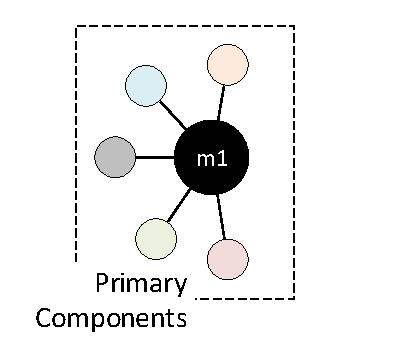
\includegraphics[width=\textwidth]{k0}
        \caption{No replication, K = 1.}
        \label{fig:datachainsingle}
    \end{subfigure}
    ~ %add desired spacing between images, e. g. ~, \quad, \qquad, \hfill etc. 
      %(or a blank line to force the subfigure onto a new line)
    \begin{subfigure}[b]{0.25\textwidth}
        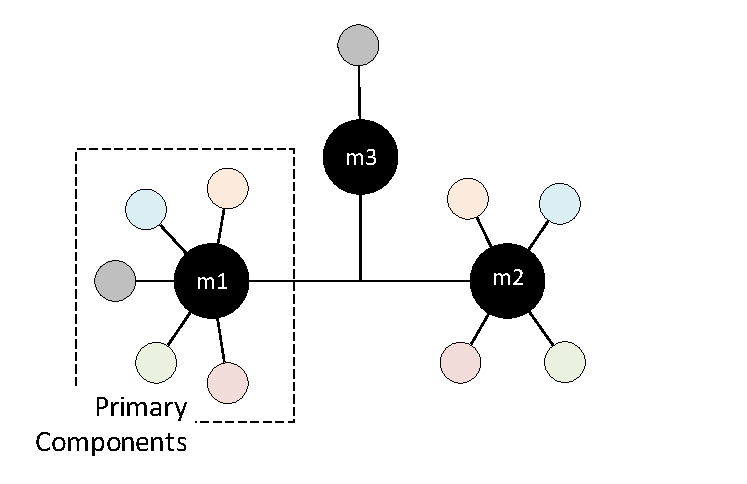
\includegraphics[width=\textwidth]{k1}
        \caption{With replication, K = 2.}
        \label{fig:datachainmulti}
    \end{subfigure}
%     ~
%         \begin{subfigure}[b]{0.3\textwidth}
%         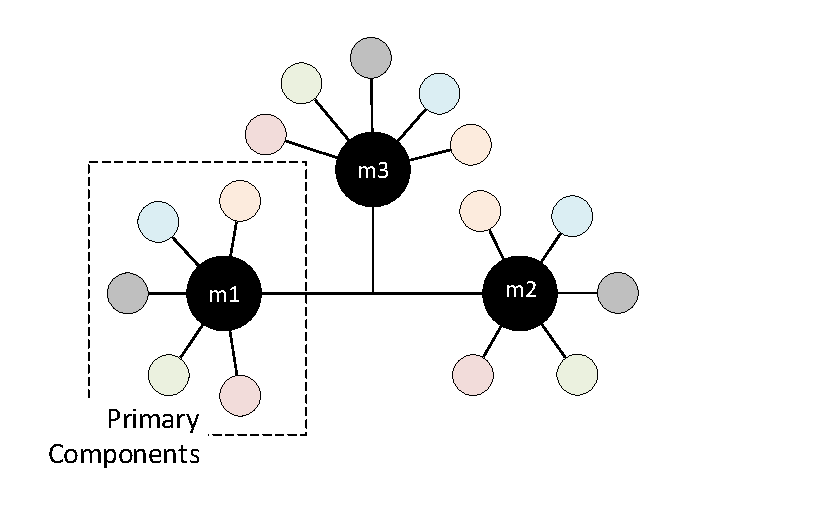
\includegraphics[width=\textwidth]{k2}
%         \caption{With Replication, K = 3}
%         \label{fig:datachainsingle}
%     \end{subfigure}
    \caption{Allocation of components.}
    \label{fig_comp_replications}
\end{figure}

In the case that the application reliability could be met with less replications, there is no need to keep unnecessary component replicas in the system. To this end, the optimization algorithm imposes soft constraints for $k>1$, which implies replicas can be allocated with \textit{overlapping}, that is, the same components can be allocated on the same node. In this case, redundant components should be discarded by design since the reliability does not improve as a result of additional replicas on the same node.

\subsection{Timing Constraints}
The timing constraints ensure that the response times of the tasks realizing the distributed application meet their deadlines. Furthermore, they ensure that the cause-effect chains satisfy their respective end-to-end timing requirements, for all possible failure-modes of the system. The constraints are formulated as logical constraints in the ILP problem, as explained in the rest of this subsection.

\subsubsection*{Tasks Deadline Constraints}
The following pseudo-code illustrates how the ILP logical constraints of the tasks deadlines are prepared. It explores all possible set of components combinations (or partitions) that can potentially be allocated to a node. And only the sets that are schedulable are asserted as constraints in to the optimization problem, which is explained as follows: Line (1) identifies the power set of the components $Par$, followed by synthesis of tasks models of each partition. Line (2) checks the tasks models' schedulability and returns a matrix $M^T$ that indicate schedulability, which is \textit{true} if the task model is schedulable and \textit{false} if not schedulable. Line (3) generates an ILP partition expression $E$ for each node, then Line (4-6) asserts the expressions to hold in the optimization for the partitions that are schedulable.
\begin{algorithm}
\caption{Generate task partitions constraints.}\label{alg_partition}
% \algsetup{
% linenosize=\small,
% linenodelimiter=.
% }	
\renewcommand{\algorithmicrequire}{\textbf{Input:}}
%\renewcommand{\algorithmicensure}{\textbf{Output:}}
\begin{algorithmic}[1]
\Require $C,M$
\Ensure Optimization Satisfies Tasks Deadlines, $D$
\State $Par \Leftarrow 2^C$	
\State $M^T\Leftarrow isSched(Par, M)$
\State $E\Leftarrow MilpParExp(x)$
\ForAll{$m \in M$}
	\State $assertOR(M^T_m, E_m, true)$
\EndFor
\end{algorithmic}
\end{algorithm}

In general, the number of potential logical constraints grow exponentially, which is in $2^{|C|}*|M|$. However, the effective logical constraints that are eventually asserted are much lower, for two main reasons: 1) a portion of the tasks models are not schedulable, therefore eliminated from the power set, due to CPU utilization exceeding the bound, not satisfying response time of either task in the partition; ii) a task model can be a super set of other tasks model. In this case, only the super model is checked, hence reducing pre-optimization time and logical constraints asserted in the solver.

\subsubsection*{Cause-effect Chains Constraints}
These constraints ensure that the cause-effect chains $\Gamma$ meet their respective end-to-end requirements $\mathrm{E2eReq}$. Similar to the previous constraints, the cause-effect chain constraints are logical assertions, which must be fulfilled by the optimal solution. The following pseudo-code illustrates how the ILP logical assertions are synthesized from the input models. 

% A cause-effect chain may consist of two or more tasks, and depending on the eventual allocation of the tasks to nodes, the chain could be hosted on a standalone node, distributed across multiple nodes. 
The pseudo-code contains three main parts: i) the first part in Line (2) identifies the different deployment cases of the cause-effect chains over a set of nodes $M$; ii) the second part in Line (3-5), checks the schedulability of a deployable cause-effect chain $\phi$ against the Reaction or Age delays  \cite{mubeen2013support} and returns its schedulability matrix $M^\Gamma$, with values $true$ if schedulable and $false$ if not schedulable. For a schedulable $\phi$, Line (5) constructs a conjunctive ILP expression that indicates the existence of at least one schedulable $\phi$ that satisfies the end-to-end requirement imposed on $\gamma$; iii) the last part in Line (7) asserts the ILP logical OR expressions for each $\gamma$.
\begin{algorithm}
\caption{Generate constraints on the cause-effect chains.}\label{alg_causeeffectchains}
\begin{algorithmic}[1]
\Require $\Gamma,M$
\Ensure Optimization Satisfies End-to-end Requirements of Cause-effect Chains
\ForAll{$\gamma \in \Gamma$}
\State $\Phi\leftarrow Unique(C^{T_\Gamma}_r, M)$ 
	\ForAll{$\phi \in \Phi$}
    \State $M^\Gamma\Leftarrow isSched(\phi, M)$
    \State $depExp\Leftarrow depExp \lor sched(M^\Gamma, true)$
    \EndFor
	\State $assert(depExp)$
\EndFor
\end{algorithmic}
\end{algorithm}


\section{Evaluation}\label{sec_evaluation}
In this section, we evaluate the proposed approach using  synthesized automotive applications that conform  to the automotive benchmark proposed by Kramel et al.~\cite{Kramer2015RealFree}. The number of runnables, timing specification and activation patterns within the cause-effect chains are also selected according to the benchmark. In order to show the scalability of our approach and to assess the scope of its applicability in practice, in some cases, we use higher specifications standard  than what is indicated in the benchmark, e.g., the maximum number of activation patterns is extended from three to four.

In the rest of the section, we describe the setup and method of evaluation, followed by discussion of the evaluation results.

%\subsection{Preparation}
\subsection{Setup}
The evaluation setup consists of three hardware platforms with different computing capacities, i.e., processing speed and memory size as shown in Table~\ref{tbl_hardwaremodel}. The evaluation on different platforms can be used as performance indicator and also to identify performance bottlenecks in the model. HP EliteBook and Lenovo 20378 are personal computers with core-i5 and core-i7 processors, respectively, whereas PowerEdge is a workstation with much higher processing and memory specification than the personal computers.
\begin{table}[h]
\centering\small
\begin{tabular}{@{}p{0.25\columnwidth}p{0.275\columnwidth}llll@{}}
\toprule
Hardware Model  & Pro. Model & \rotatebox{70}{\#Pro.} & \rotatebox{70}{\#Core} & \rotatebox{70}{Cache} & \rotatebox{70}{RAM}\\ \midrule
$^1$HP EliteBook & $^3$Core i5, 2.2GHz & 1 & 2 & 3M & 8G \\ 
Lenovo 20378 & $^4$Core i7, 2.6GHz & 1 & 4 & 6M & 16G\\ 
$^2$PowerEdge & $^5$Xeon(R), 2.4GHz & 24 & 6 & 15M & 256G\\
\bottomrule
\end{tabular}
\caption{Summary of the Hardware Specifications.\\
\footnotesize{$^1$HP EliteBook 840 G2, $^2$PowerEdge R730 Rack Server}\\
\footnotesize{$^3$Intel® Core™ i7-4720HQ @ 2.60GHz, $^4$Intel® Core™ i7-4720HQ @ 2.60GHz $^5$Intel(R) Xeon(R) CPU E5-2620 v3 @ 2.40GHz}}
\label{tbl_hardwaremodel}
\end{table}

\subsubsection{Software Application Benchmark} In order to evaluate the proposed approach on different ranges of applications, we automatically generate synthetic examples that comply with the automotive benchmark~\cite{Kramer2015RealFree}. The examples denote simple to complex automotive functions such as reverse-parking assistance system and engine control system. For simplicity, we identify three classes of applications with different sizes and complexity, shown as tuple $(c, r, t, g)$, respectively for the number of software components, runnables, tasks, and cause-effect chains. Table \ref{tbl_appsspec} shows the range of values used in the applications for evaluation. 
\begin{table}[h]
\centering\small
\begin{tabular}{@{}llll@{}}
\toprule
Parameter  		& Spec.-I  & spec.-II & spec.-III\\ 
\midrule
components, $c$		& $\leq 10$	& $\leq 15$ 	& $> 15$\\ 
runnables, $r$		& $\leq 50$	& $\leq 100$ 	& $> 100$\\
tasks, $t$ 			& $\leq 30$ & $\leq 60$ 	& $> 60$\\
cause-effect chains, $g$ & $\leq$ 30 & $\leq$ 40 & $> 60$\\ \midrule
activation-pattern	& \multicolumn{3}{c}{$[2,3,4]$}\\ \midrule
share of activation-patterns	& \multicolumn{3}{c}{$[0.7, 0.2, 0.1]$}\\
\bottomrule
\end{tabular}
\caption{Specification of the Applications for Evaluation.}
\label{tbl_appsspec}
\end{table}

\subsubsection{Platform Benchmark} The specification of nodes can be obtained from simulation, vendor product specification and  experience. Figure~\ref{tbl_nodesspecs} shows the range of values that are used in the nodes' specification. In the experiment, the values are randomly generated while respecting the benchmark.
\begin{table}[h]
\centering\small
\begin{tabular}{@{}llll@{}}
\toprule
Parameter  		& Range\\ 
\midrule
nodes							& $4-10$\\
power consumption (Watt), $p$ 	& $10 - 200$\\
failure-rate (/Mhr), $\lambda$ 	& $10^4 - 10^{-2}$\\
speed factor, $hz$			 	& $0.0 - 1.0$\\
\bottomrule
\end{tabular}
\caption{Range of Values for the Specification of Nodes.}
\label{tbl_nodesspecs}
\end{table}

\subsection{Result}
We conduct three experiments that assess the proposed approach for scalability in terms of \textit{allocation time}. The allocation time is defined as the time required to prepare and solve the allocation problem using the proposed ILP method. Furthermore, we show resource efficiency in terms of saving nodes (i.e., using smaller number of nodes). The experiments consist of: i) varying the size of applications in order to observe the effect of increasing components, runnables and tasks in the system, ii) varying the complexity of applications in order to observe the effect of cause-effect chains in the system, and iii) varying the replications. The experiments are discussed in detail in the next subsection.

A preliminary analysis of the evaluation indicates a successful termination of the allocation for Spec-I\&II of the applications. Whereas for Spec-III, the allocation problem is intractable. In fact, it took days on the PowerEdge machine and many times it did not terminate successfully. Therefore, the experimental results that are shown in this paper are conducted on the Spec-I\&II classes. 
\begin{figure*}
    \centering
    \begin{subfigure}[b]{0.525  \textwidth}
        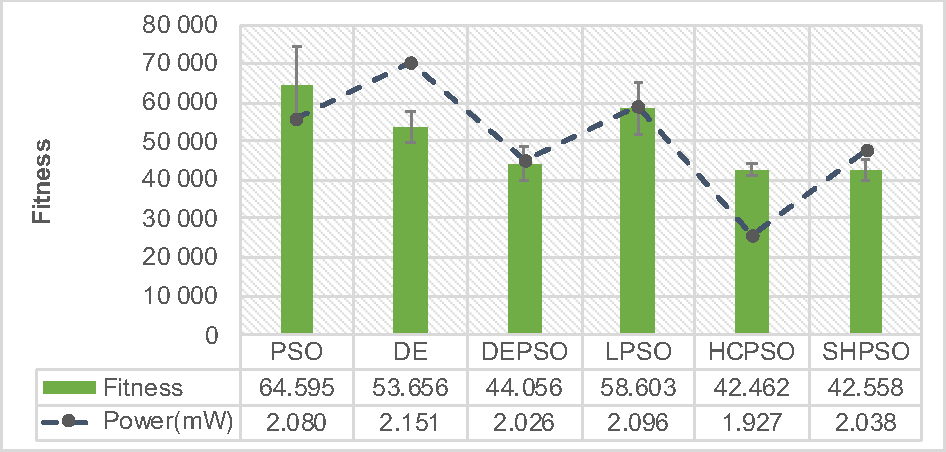
\includegraphics[width=\textwidth]{img/fitness_c20_g30_m10.pdf}
        \caption{Fitness and Power Consumption.}
        \label{fig_util}
    \end{subfigure}
    ~%\hspace{-0.4cm}
        \begin{subfigure}[b]{0.45\textwidth}
        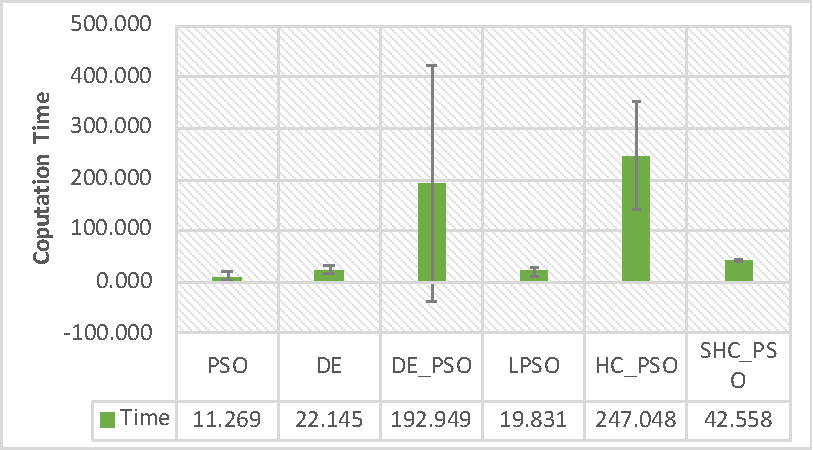
\includegraphics[width=\textwidth]{img/time_c20_g30_m10.pdf}
        \caption{Computation Time}
        \label{fig_power}
    \end{subfigure}
    \caption{Allocation of Software Application $(N_c=20,N_r=200,N_\Gamma=30)$ on $N_m$ number of Heterogeneous Nodes using Different Optimization Methods.}
    \label{fig_util_power}\vspace{-0.2cm}
\end{figure*}



\begin{figure}[t!]
\centering
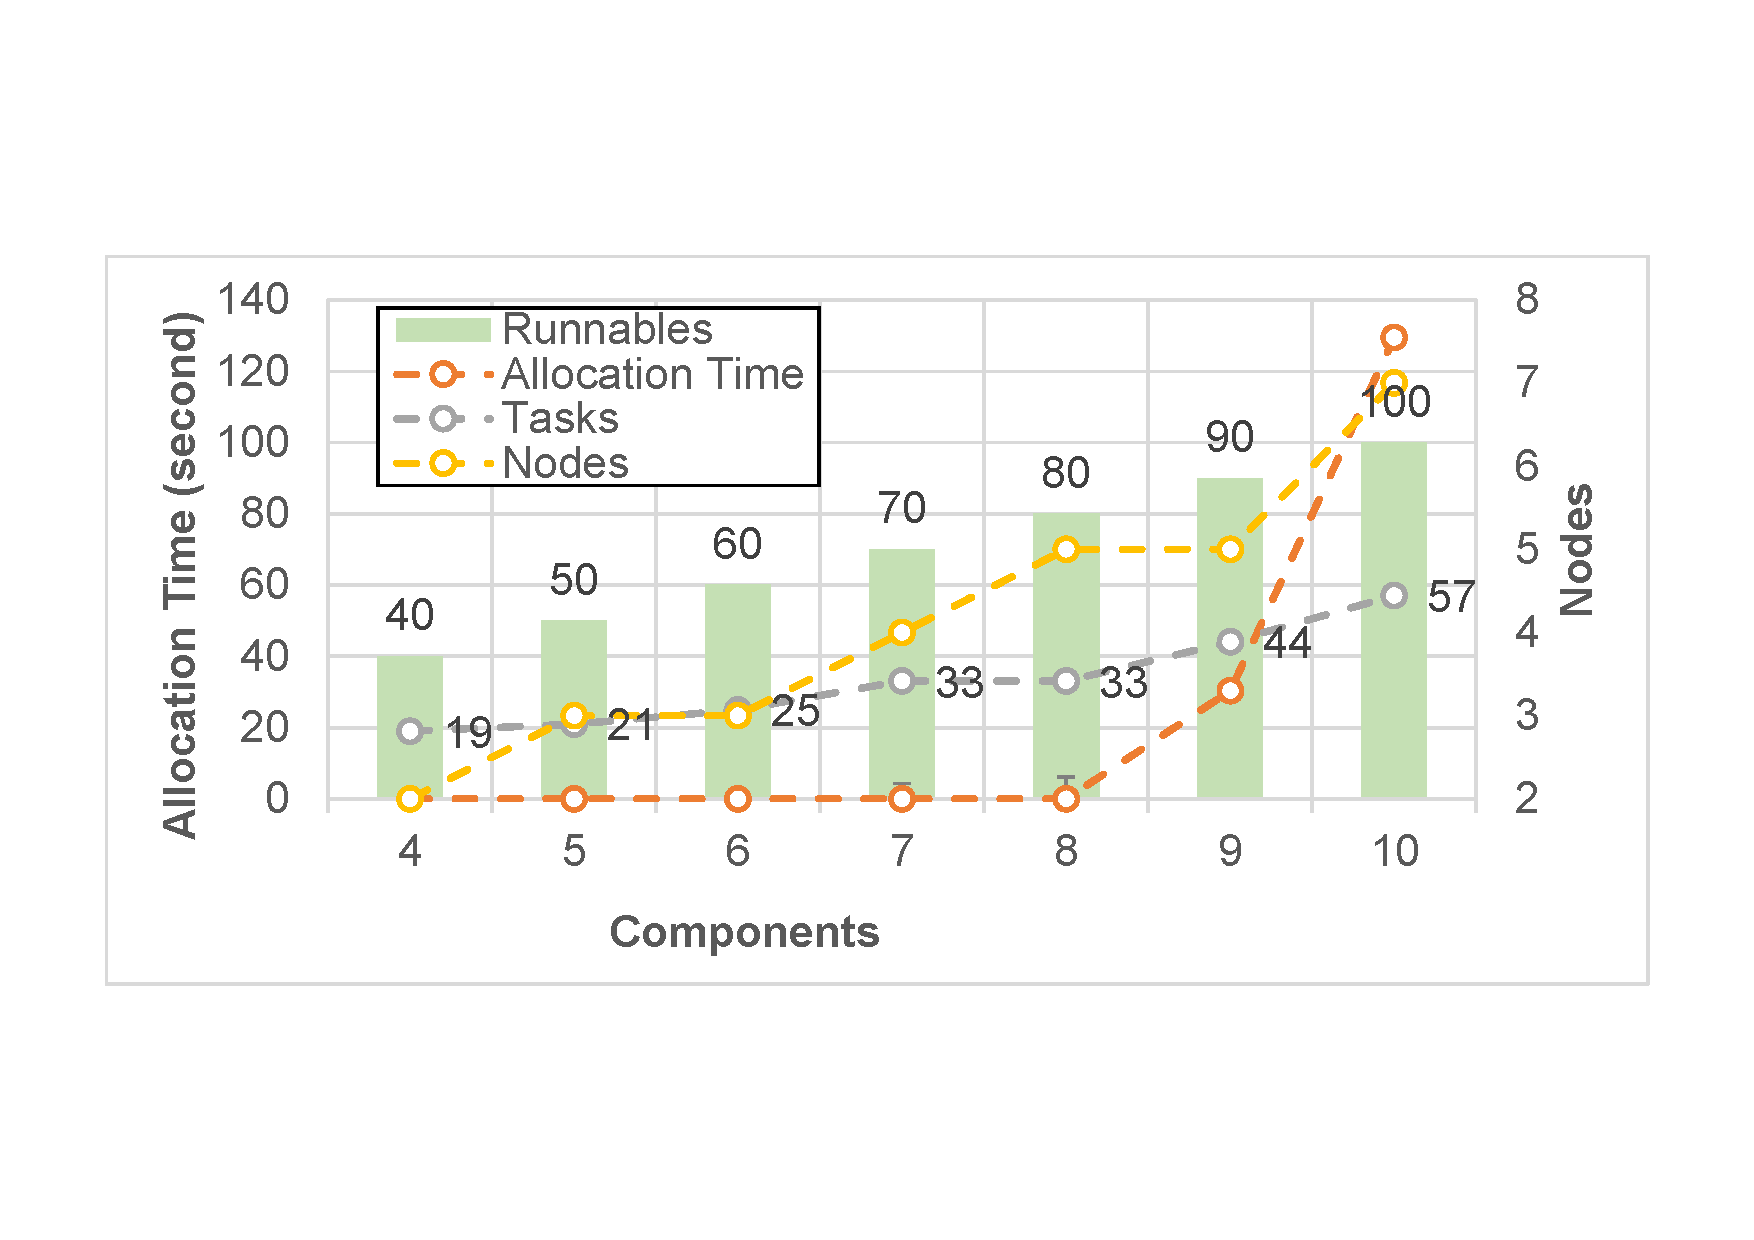
\includegraphics[width=0.7\linewidth]{increasing_components}
\caption{Effect of Varying the Application Size on the Allocation Time and Number of Utilized Nodes.}
\label{fig_increasing_components}
\end{figure}

\subsubsection{ILP Evaluation}
\paragraph{Varying the Size of Application} 
This refers to increasing the number of software components, as well as runnables, tasks, and cause-effect chains in the system. Figure~\ref{fig_increasing_components} shows the effect of increasing the size of an application from $(c4,r40,t19,g30)$ to $(c10,r100,t57,g60)$ on the allocation time and  the number of nodes utilized. The applications are allocated to a pool of 8 heterogeneous nodes sharing a single network and with specifications shown in Table~\ref{tbl_nodesspecs_exp}. The specifications are generated randomly, with uniform distribution, within the scope of Table~\ref{tbl_nodesspecs}.
% Please add the following required packages to your document preamble:
% \usepackage{booktabs}
\begin{table}[]
\small
\begin{tabular}{@{}llllllll@{}}
\toprule
Application & Measure & PSO & LPSO & DE & DEPSO & HCPSO & SHPSO \\ \midrule
App1 & Mean &  &  &  &  &  &  \\
 & Std.Dev. &  &  &  &  &  &  \\
App2 &  &  &  &  &  &  &  \\ \bottomrule
\end{tabular}
\end{table}

\begin{figure*}
    \centering
    \begin{subfigure}[b]{0.4  \textwidth}
        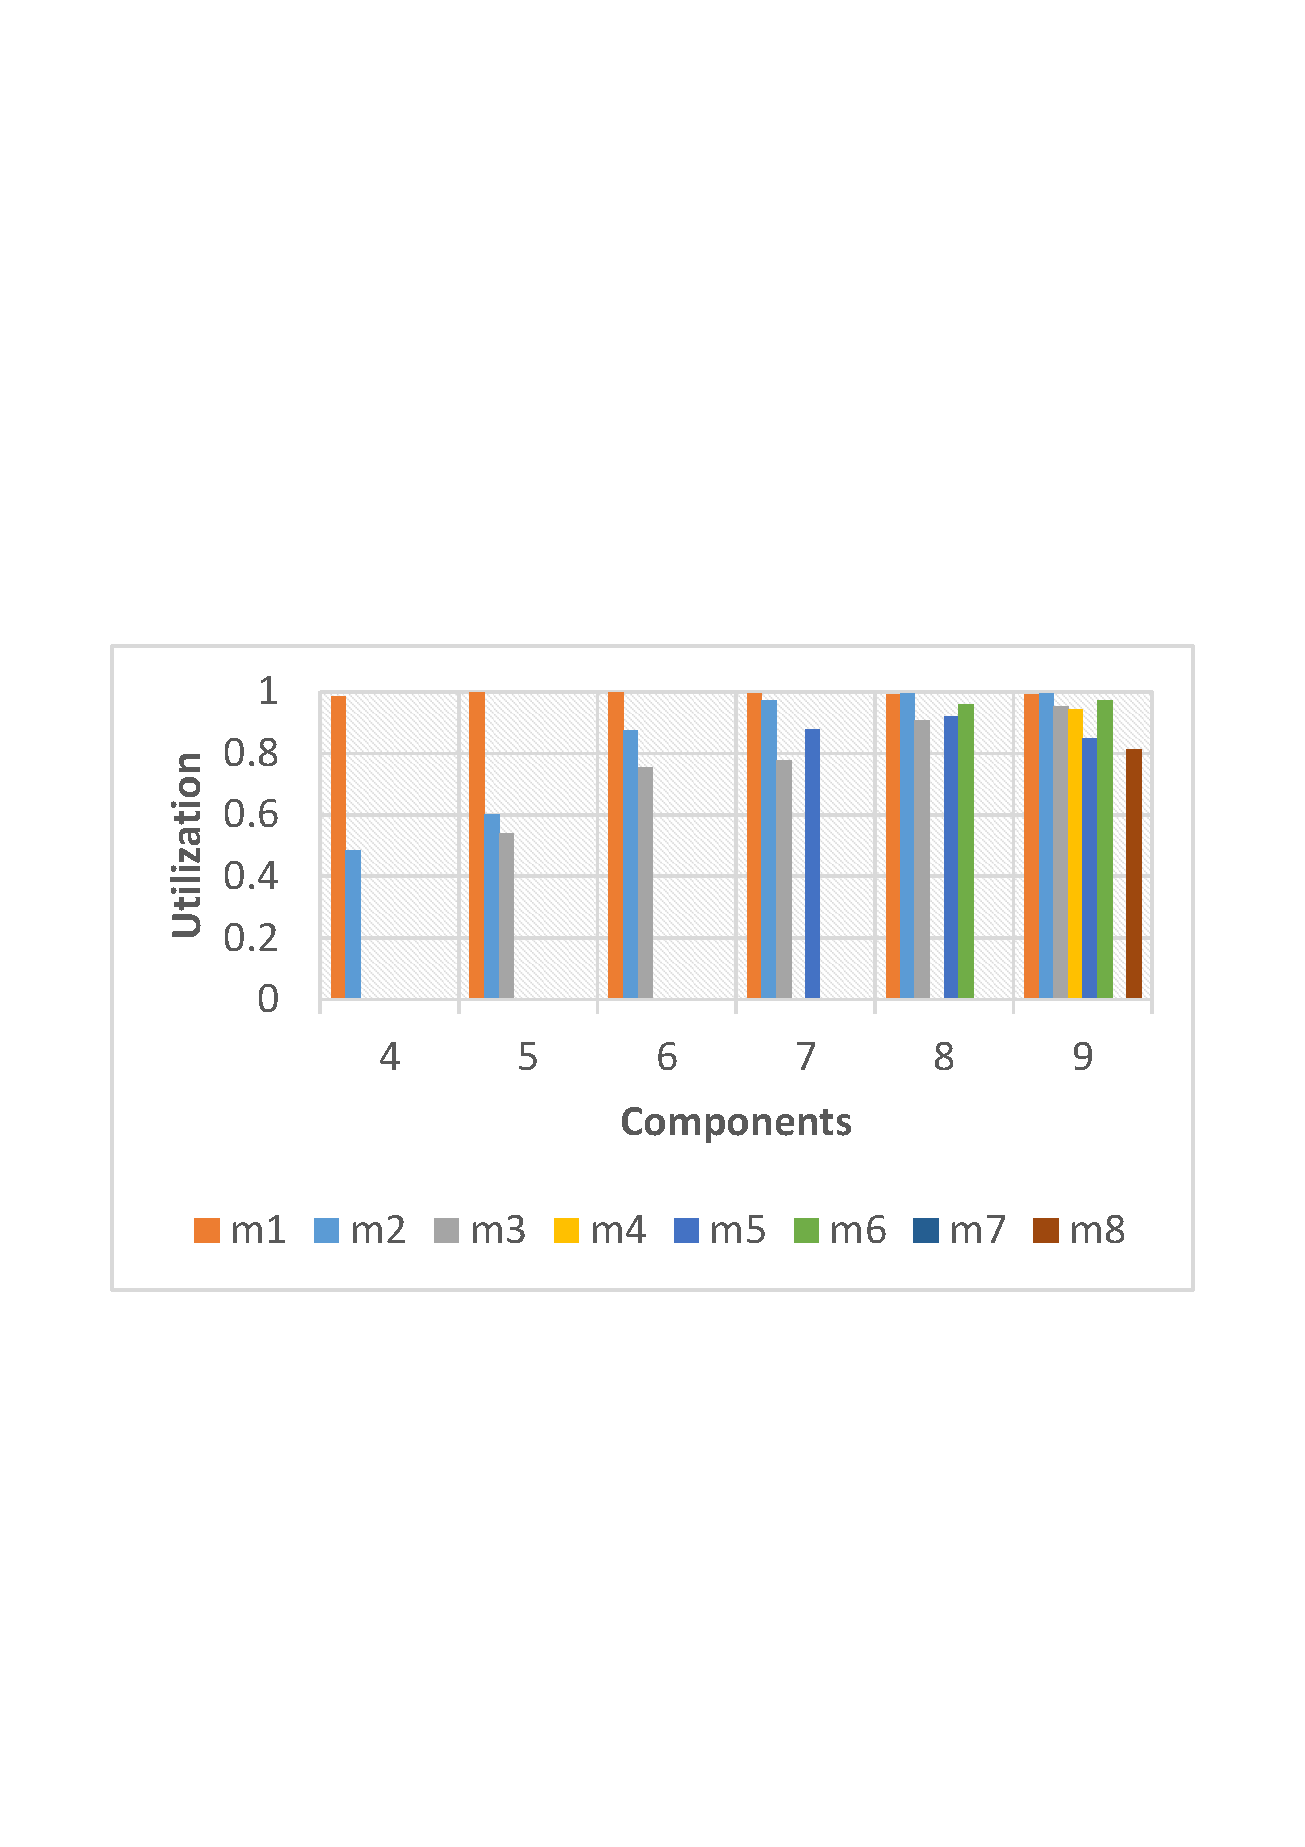
\includegraphics[width=\textwidth]{util}
        \caption{Utilization of Nodes.}
        \label{fig_util}
    \end{subfigure}
    ~%\hspace{-0.4cm}
        \begin{subfigure}[b]{0.4\textwidth}
        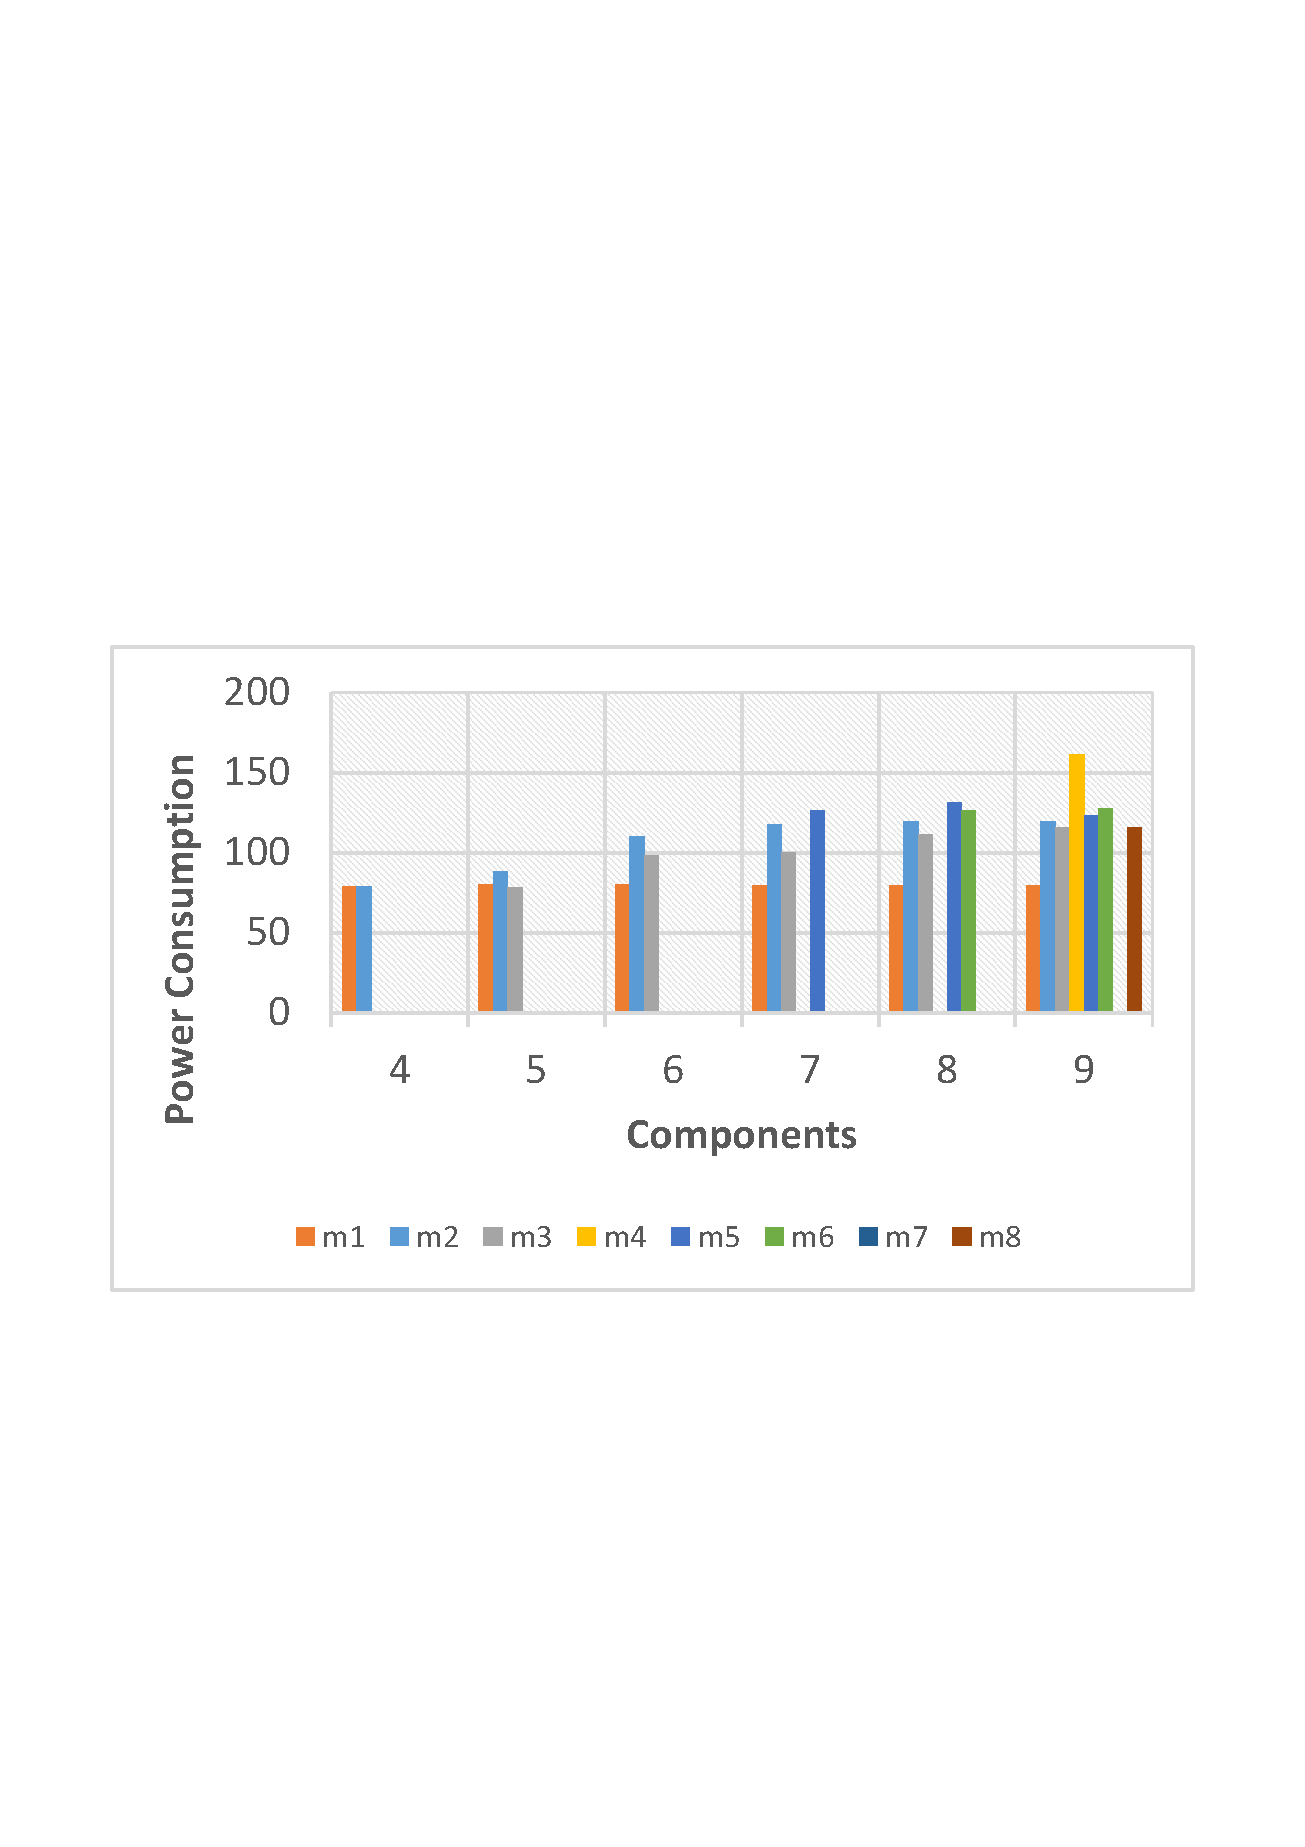
\includegraphics[width=\textwidth]{power}
        \caption{Power Consumption of Nodes.}
        \label{fig_power}
    \end{subfigure}
    \caption{Allocation of Applications on Heterogeneous Nodes.}
    \label{fig_util_power}\vspace{-0.2cm}
\end{figure*}

The CPLEX solver returns an optimal solution for the application $(c8, r80,t44,g30)$ within 6.06 sec. The allocation time increased sharply to 30.3 sec and 129.4 sec respectively for 9 and 10 components. Even if not indicated in this chart, the solver, the solver returns an optimal solution within 45 min for components reaching 15 on the PowerEdge machine and OutOfMemory error on the Lenovo and HP machines. Figure~\ref{fig_util} and Figure~\ref{fig_power} show the utilization and power consumption on each node for the different application sizes. The optimal allocation, in the general case, favor nodes with higher processor speed and lower power consumption specifications.

\paragraph{Varying the Number of Cause-effect Chains} 
In order to observe the effect of increasing the cause-effect chains on the allocation time, we vary the number of chains in the application from 10 to 60, which is consistent with the benchmark~\cite{Kramer2015RealFree}. The share of activation patterns also increases proportionally with the ratio $1:[0.7, 0.2, 0.1]$, respectively, for two, three, and four activation patterns. For instance, out of 10 cause-effect chains, there are 7 chains (with two activation patterns), 3 chains (with three activation patterns), and 1 chain (with four activation patterns). The experiment is conducted on two cases of schedulability analysis, namely response time analysis (RTA) and utilization bound (UB), and their result is shown in  Figure~\ref{chart_cause_effect_chain} for increasing number of chains.
\begin{figure}[h!]
\centering
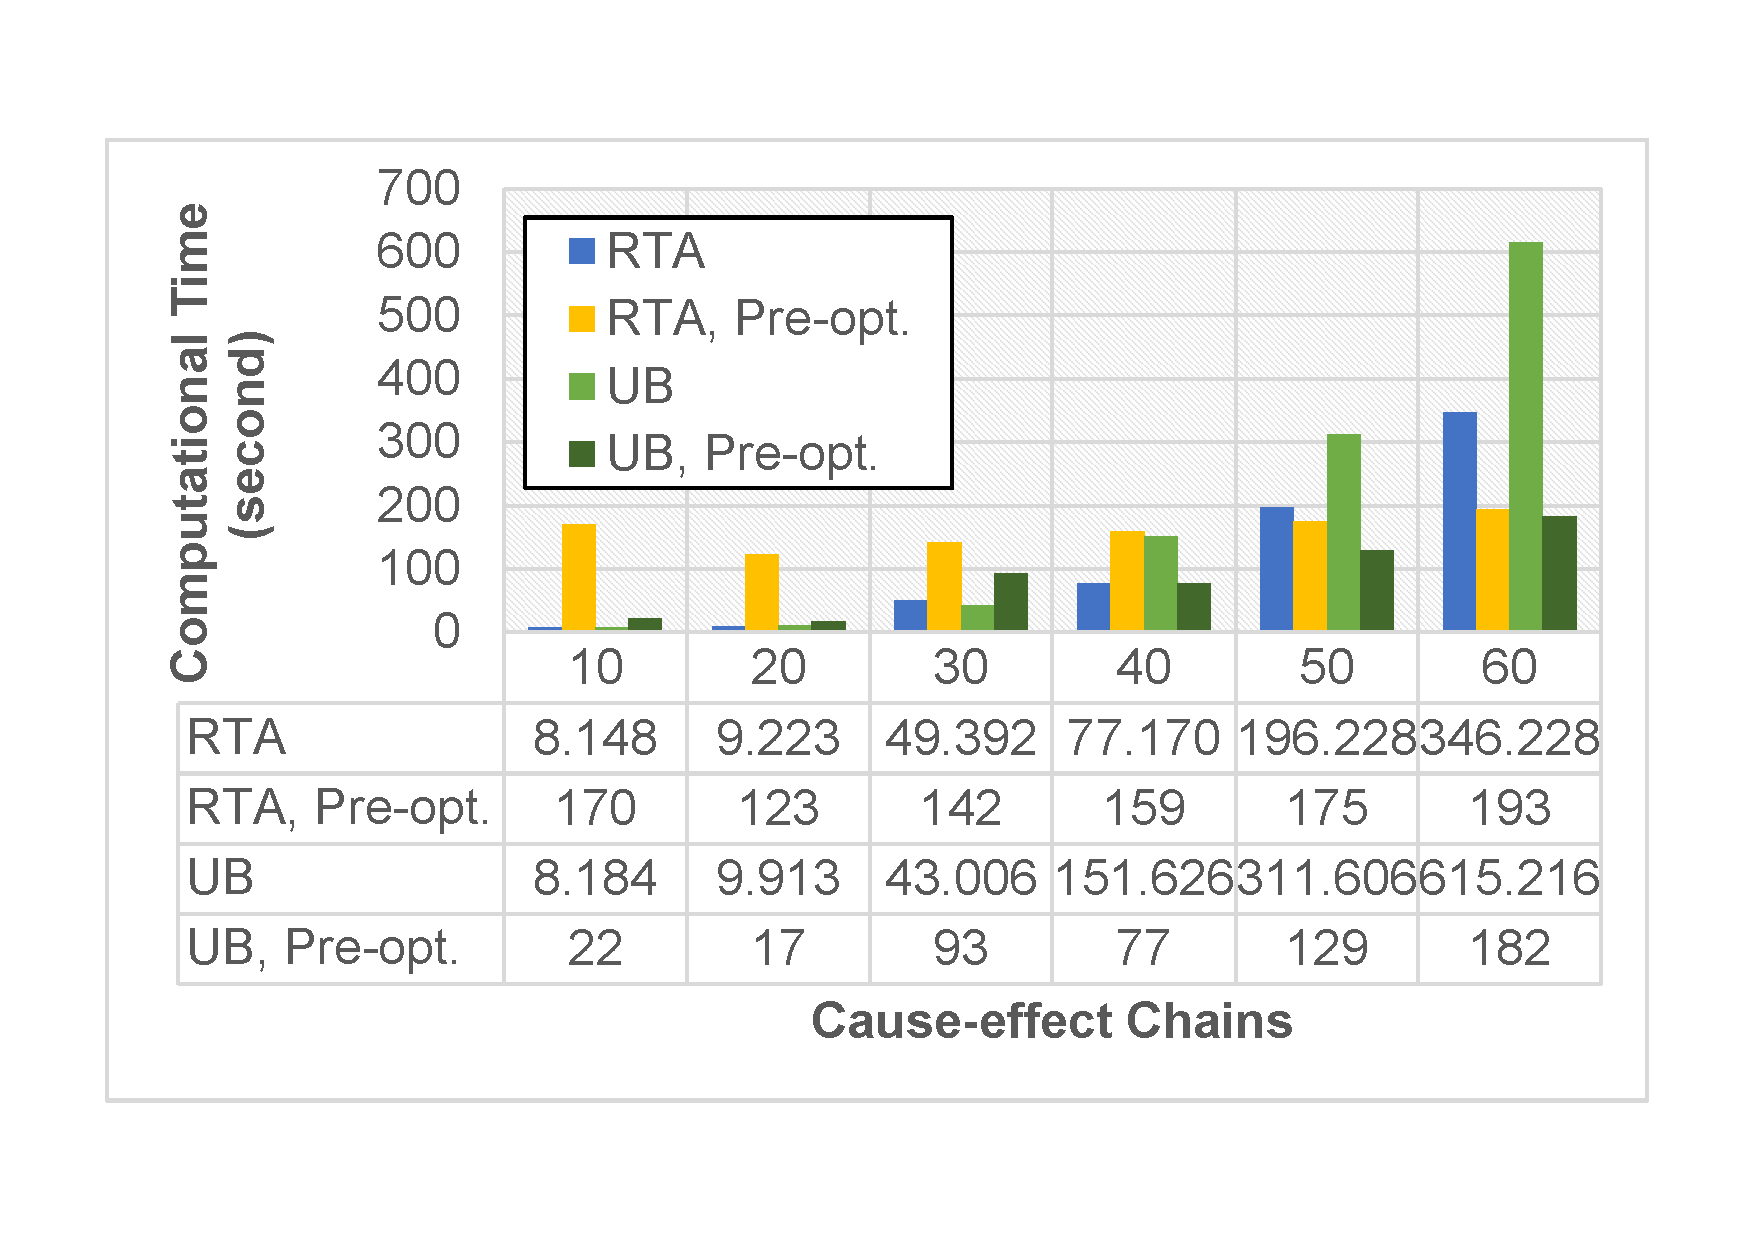
\includegraphics[width=0.7\linewidth]{increasing_cause-effect_chains}
\caption{Effect of Increasing Cause-effect Chains (under RTA and UB) on the Allocation Time.}
\label{chart_cause_effect_chain}\vspace{-0.4cm}
\end{figure}

The figures in the data table show an exponential growth of allocation time whenever the cause-effect chains are increased linearly for a specific application, in both cases of schedulability analysis. In the case of RTA, the overhead in the pre-optimization is higher than the overhead in the optimization for 50 or less chains. Whereas in the UB case, the computational time of pre-optimization is almost always less than the computational time of the optimization. 
The results are consistent with our expectation that the RTA computation, in the preparation of the timing assertions, is expensive, albeit provides schedulable tasks allocation based on the fixed-priority scheduling policy. In contrast, the UB computation time is relatively low; however, the search space gets larger due to more and more feasible tasks partitioning and chains fulfilling the timing constraints. As a result, the optimization time in the case of UB is usually higher as compared to the case of RTA. Therefore, for applications with chains not more than 40 and naive scheduling assumption using UB, the experiments favor the UB assumption. Whereas, the allocation with the RTA assumption should be selected for applications with exact scheduling requirements. Note, the scalability of this experiment should be seen in conjunction with the experiment discussed in the previous subsection.

\paragraph{Varying Replications}
In this experiment, we evaluate the allocation time of the applications with the increase in the number of replications. For the applications specification shown in Figure \ref{fig_replication}, we vary the replications from 1 to 4. 
The allocation in all applications took not more than 10 sec for replications 1 and 2. For Spec-I with replication 3 and 4, the allocation time went up close to 1 min. For Spec-III with replication 3, the allocation time went up rapidly to 30 min, and took extremely large time for replication 4 which is also the case for Application-II.
\begin{figure*}[h]
    \centering
    \begin{subfigure}[b]{0.475\textwidth}
        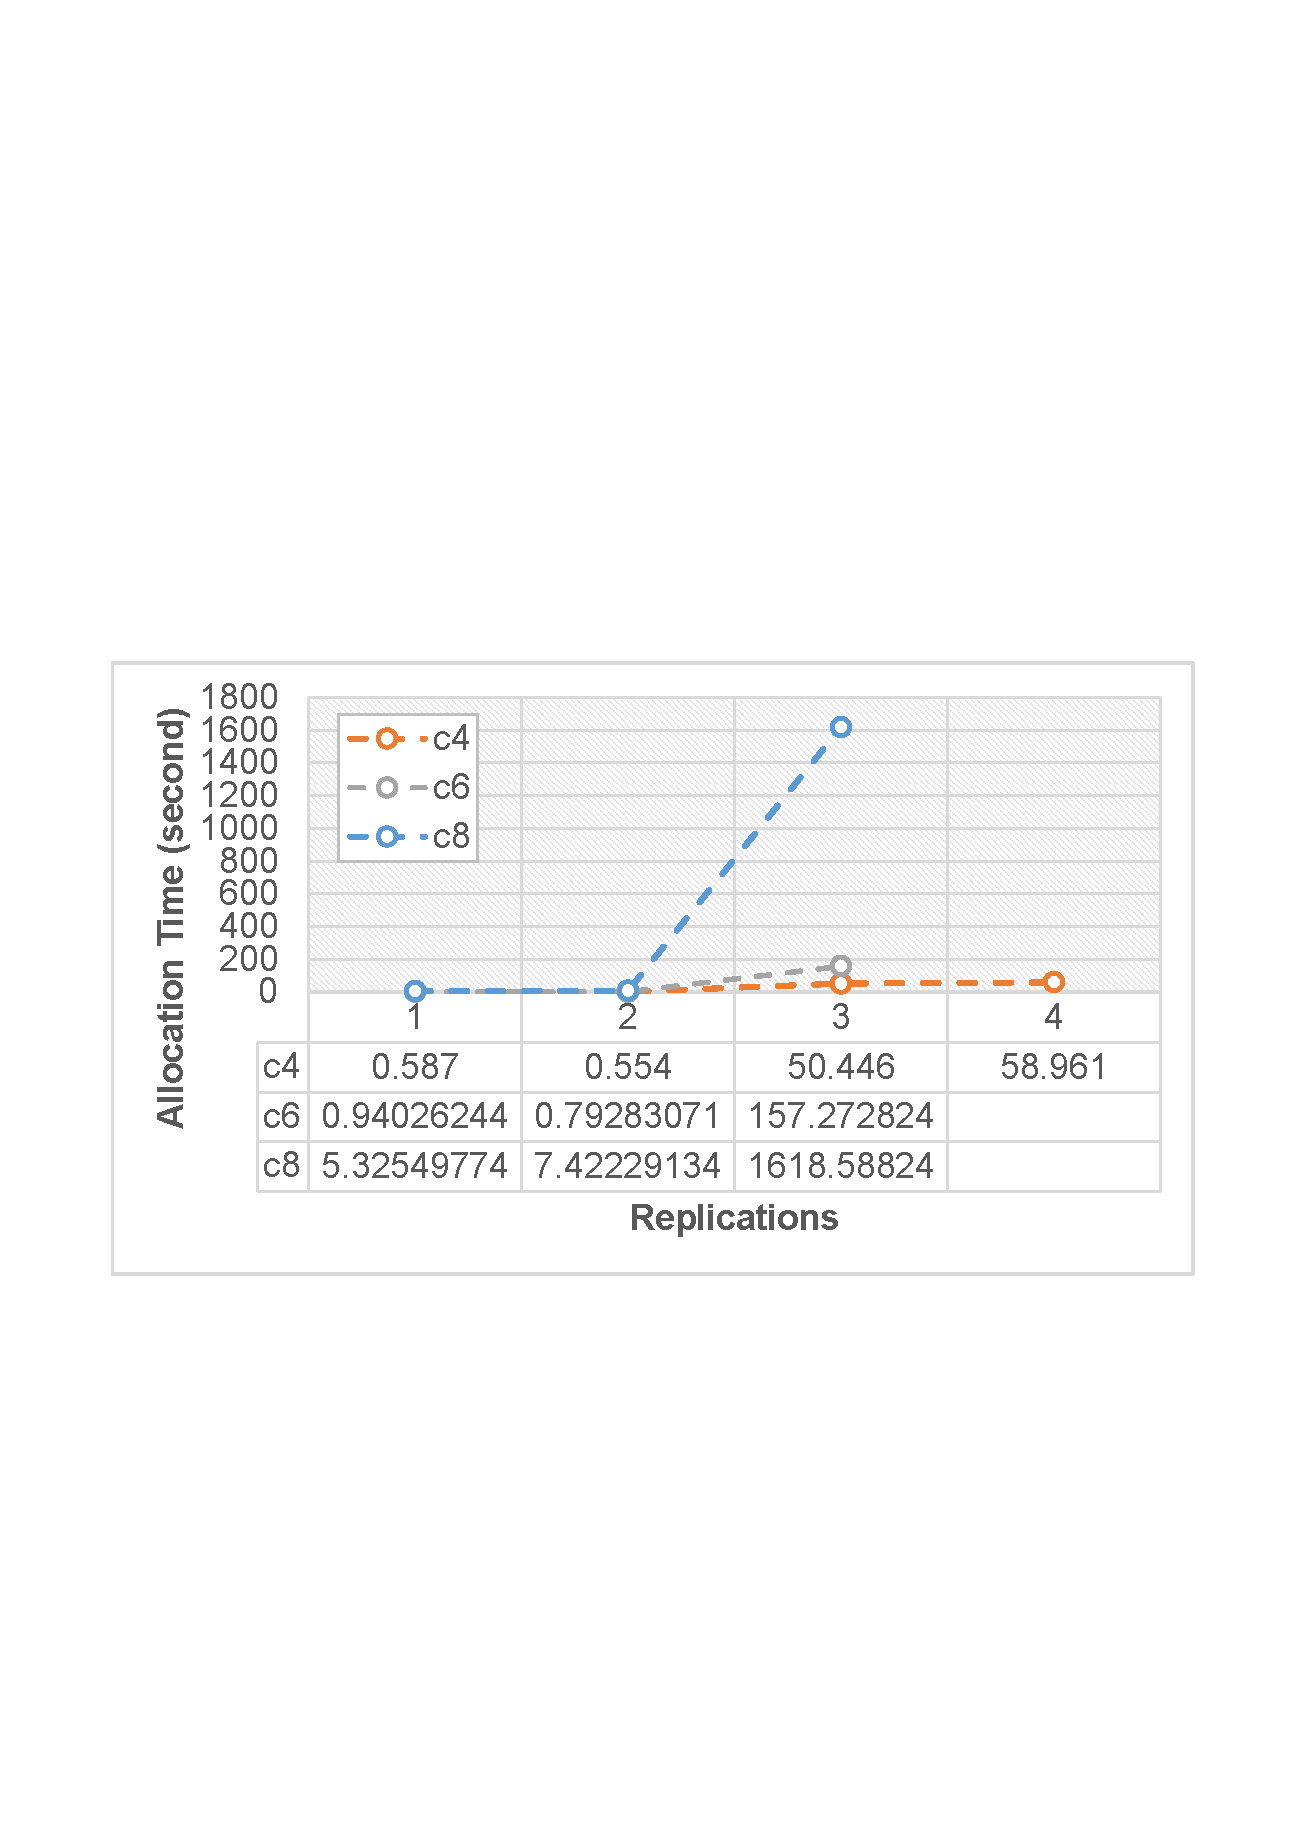
\includegraphics[width=\textwidth]{replications}
        \caption{Effect on Allocation Time.}
        \label{fig_replication_1}
    \end{subfigure}
    ~
        \begin{subfigure}[b]{0.475\textwidth}
        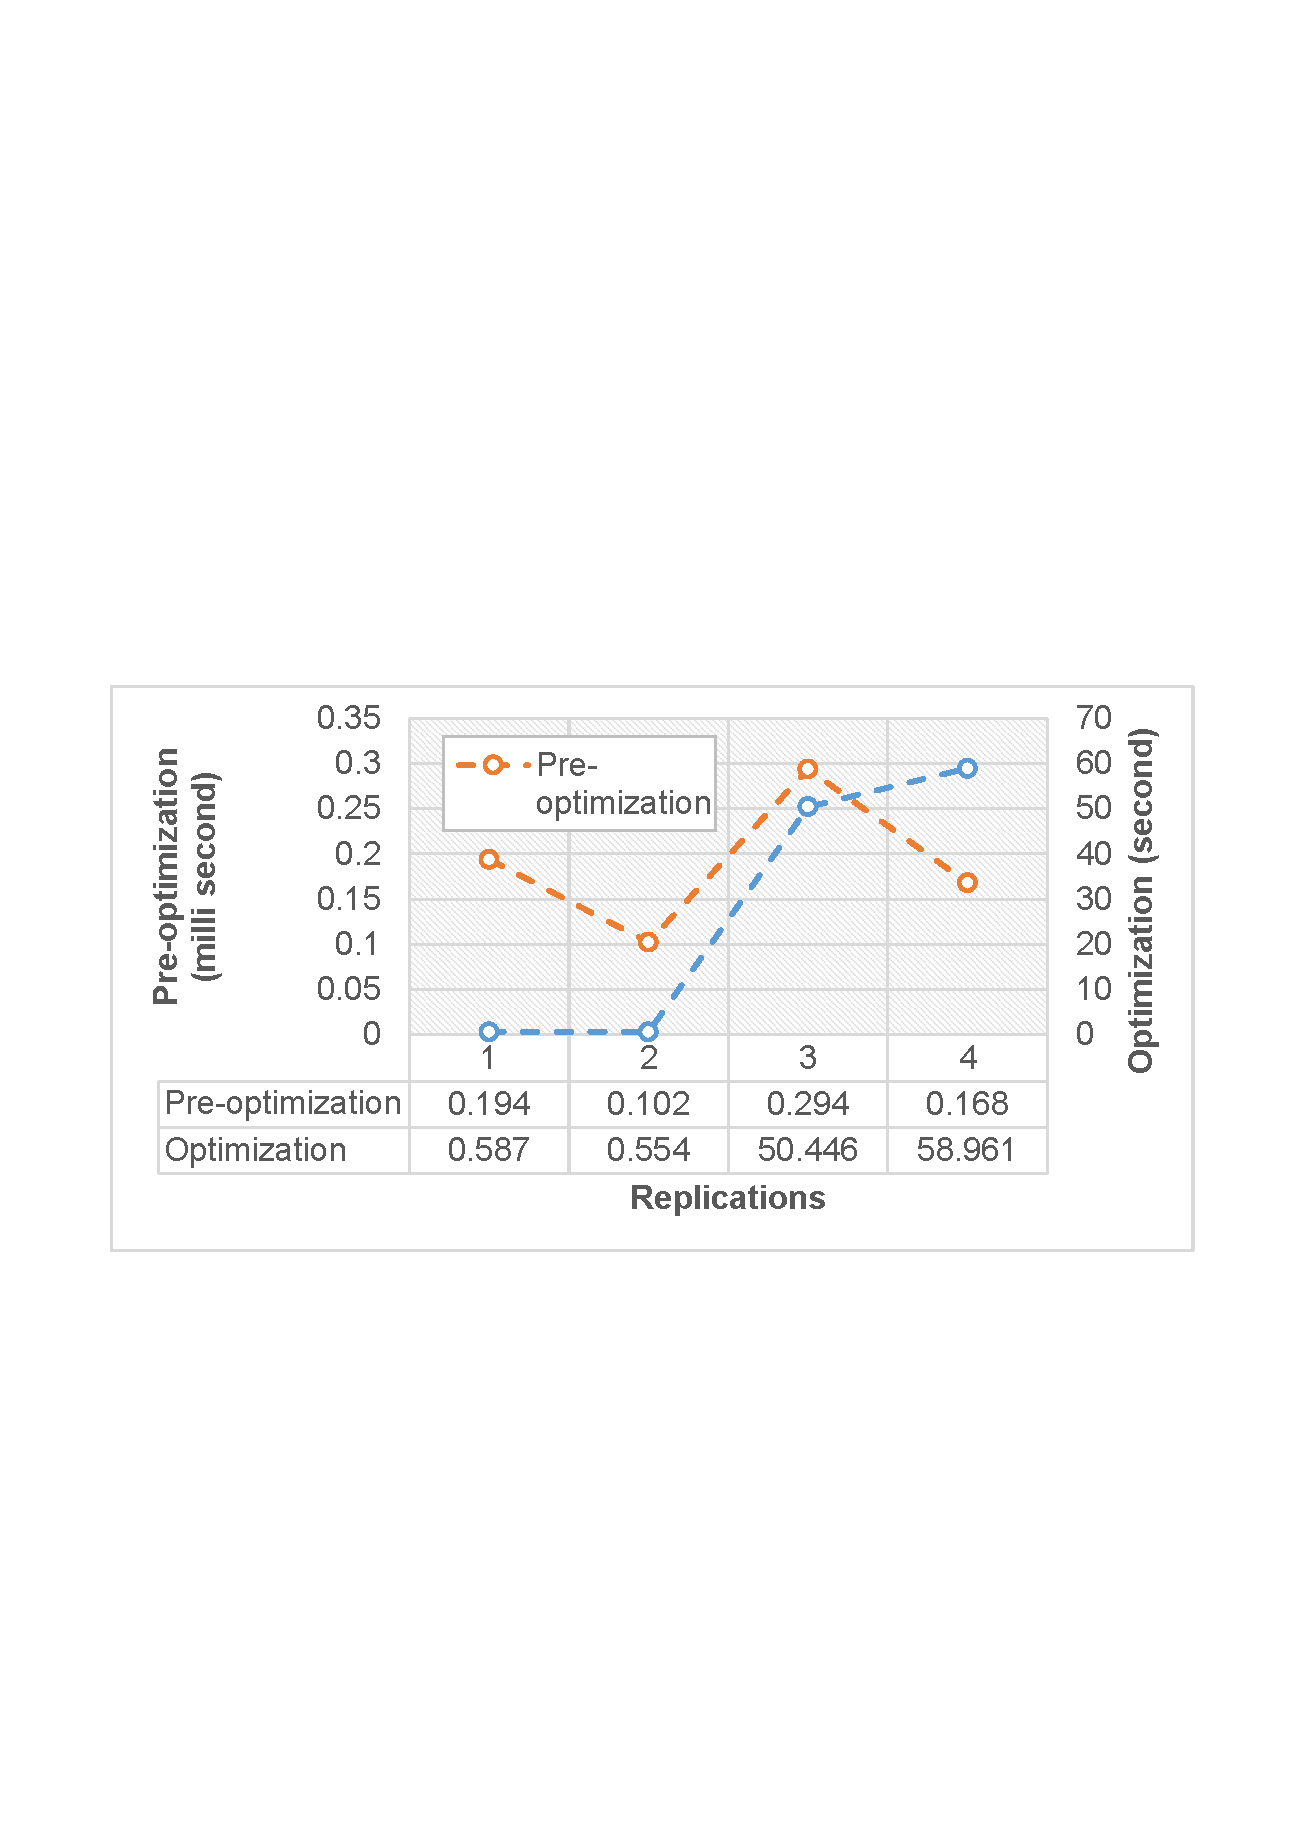
\includegraphics[width=\textwidth]{replication_comparison}
        \caption{Effect on Pre-optimization.}
        \label{fig_replication_2}
    \end{subfigure}
    \caption{Effect of Varying the Component Replications on the Allocation Time.}
    \label{fig_replication}\vspace{-0.5cm}
\end{figure*}

Figure~\ref{fig_replication_2} shows the effect of shared constraints on the overhead of replications during the pre-optimization and optimization phases of the allocation. In the pre-optimization phase, the allocation time was stable for the increased size of applications. This is due to the fixed constraints regardless of the replications. In contrast, the allocation time increases during optimization as the constraints are applied for the various combination of task partitions, cause-effect chains, and reliability states generated as the result of replications.

\subsection{Metaheuristic Evaluation}
Clearly, the ILP evaluation shows that the ILP approach does not scale to large software allocation problems, that is, that allocation time increases exponentially as the size of the software application increases. In fact, the allocation does not return results for applications consisting more than 15 software components. In this subsection, we evaluate ILP in conjunction with the PSO, DE, and hybrid PSO techniques for different problem sizes.

Table \ref{tbl_fitness_allocationtime_ilp_plus_metaheuristic} shows the fitness values and allocation time of the different algorithms for the increasing sizes of the software allocation problems. For no constraints violations, the fitness values denote the total power consumption, which is the case for the first three problems whereas it is not the case for the last three problems, thus the fitness values extremely increased as more violations are made. Furthermore, the algorithms highlighted in bold shows the benchmark for the corresponding specific problems. 

The result shows that the ILP approach returned solutions for the first three problems, in which case it becomes the benchmark for the quality assessment of the metaheuristic algorithms. Whereas, for the last three problems, ILP does not return solution, which conforms the previous ILP evaluation results. The metaheuristic results are further discussed as follows, that is with regard to solution quality and computation time.

\paragraph{Solution Quality} For the first problem, which models the smallest software allocation over heterogeneous nodes, the algorithms DE, LPSO, HCPSO, SHPSO returned the optimal results besides ILP, with zero deviations. However, DEPSO performed relatively worse but better than PSO. The same results are repeated out of the second allocation problem for the algorithms HCPSO, and SHPSO, which are optimal. In contrast, DE and LPSO performed worse followed by DEPSO, and PSO performed relatively the worst. For the third problem, no metaheuristic algorithms returned the optimal solutions on average. Furthermore, the stability of the solutions for the algorithms DE and PSO, as indicated by the standard deviations of the fitness values, are quite higher than the rest metaheuristic algorithms.
\begin{figure}[h!]
\centering
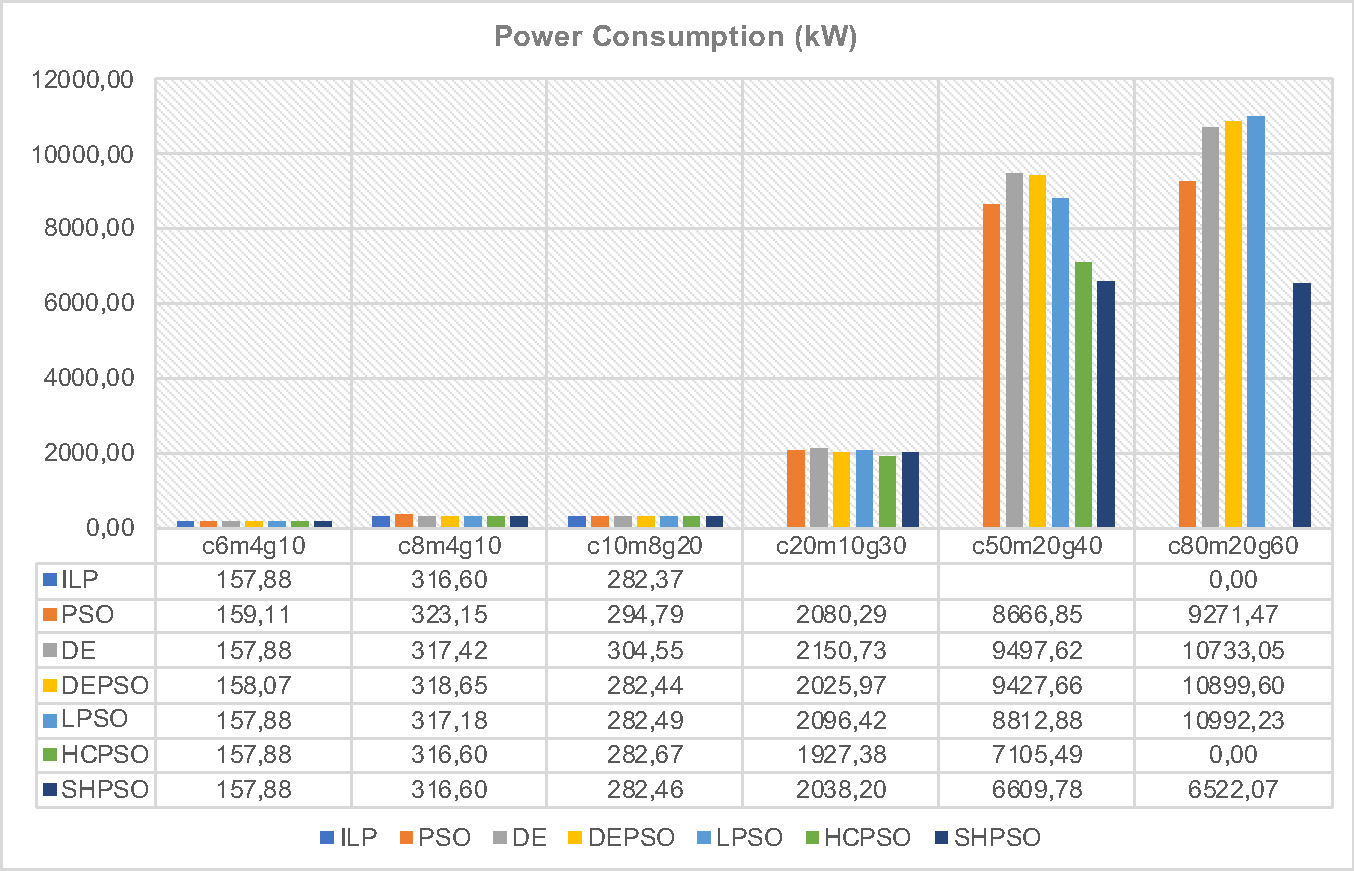
\includegraphics[width=1\linewidth]{img/power_consumption.pdf}
\caption{(Near) Optimal Power Consumption of the Different Software Allocation Problems.}
\label{fig_powerconsumption_ilp_metaheuristic}\vspace{-0.4cm}
\end{figure}

As the size of the problem further increases, that is \textit{c20m10g30} and \textit{c20m10g30}, the hybrid PSO performed the far better, with HCPSO the best followed by SHPSO and DEPSO. However, as the size of the problem further increases, that is with \textit{c80m20g60}, HCPSO did not return solutions at reasonable time. In contrast, its stochastic variant HCPSO performed the best followed by DEPSO, LPSO, and PSO, in order of their solutions quality, and DE performed the last.

\paragraph{Allocation Time} In the case of metaheuristic algorithms, the allocation time refers to the amount of time needed to return the near (optimal) result. It is calculated over a maximum of 5000 iterations (or generations) and maximum steady time of 5mins, that is, the period in which no changes are observed in the fitness values. Figure \ref{fig_allocationtime_ilp_metaheuristic} shows the allocation time of the algorithms for the problems listed in Table \ref{tbl_fitness_allocationtime_ilp_plus_metaheuristic}. ILP rapidly increased to 14sec for the problem \textit{c10m8g20} which became intractable for larger problems. Whereas HCPSO rapidly increased to 17sec for the problem \textit{c50m20g40} and became intractable for larger problems. However, for the rest of the algorithms, the allocation time did not exceed 6secs for all of the allocation problems.
\begin{figure}[h!]
\centering
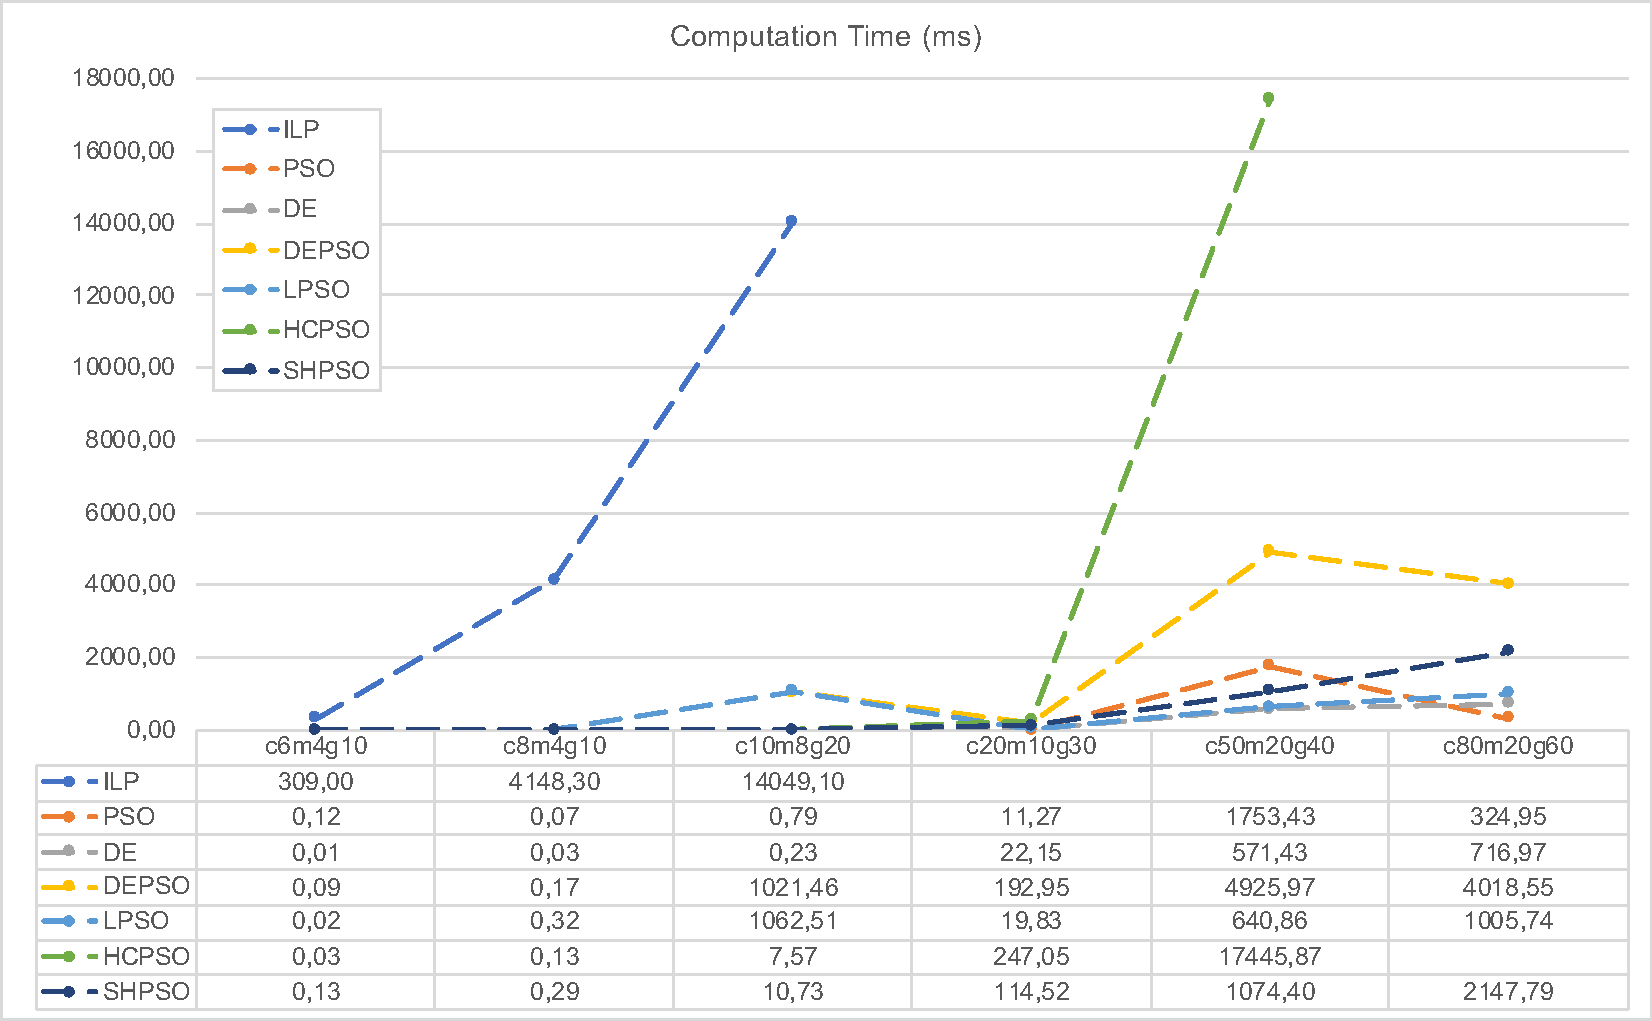
\includegraphics[width=1\linewidth]{img/time_summary.pdf}
\caption{Computation Time of the Various Algorithms for Solving Different Instances of the Software Allocation Problem.}
\label{fig_allocationtime_ilp_metaheuristic}\vspace{-0.4cm}
\end{figure}
%\begin{adjustbox}{angle=90}
\small
% Please add the following required packages to your document preamble:
% \usepackage{booktabs}

\begin{tabular}{@{}llllllllll@{}}
\toprule
Application & method & Fitness &  &  &  & power &  &  &  \\ \midrule
 &  & min & max & avg & std & min & max & avg & std \\
c6, m4,g10 & ILP & 2.28E+02 & 2.28E+02 & 2.28E+02 & 0.00E+00 & 1.58E+02 & 1.58E+02 & 1.58E+02 & 3.00E-14 \\
 & PSO & 2.28E+02 & 2.35E+02 & 2.29E+02 & 2.38E+00 & 1.58E+02 & 1.65E+02 & 1.59E+02 & 2.38E+00 \\
 & DE & 2.28E+02 & 2.28E+02 & 2.28E+02 & 3.00E-14 & 1.58E+02 & 1.58E+02 & 1.58E+02 & 3.00E-14 \\
 & DEPSO & 2.28E+02 & 2.29E+02 & 2.28E+02 & 3.08E-01 & 1.58E+02 & 1.59E+02 & 1.58E+02 & 3.09E-01 \\
 & LPSO & 2.28E+02 & 2.28E+02 & 2.28E+02 & 3.00E-14 & 1.58E+02 & 1.58E+02 & 1.58E+02 & 3.00E-14 \\
 & HCPSO & 2.28E+02 & 2.28E+02 & 2.28E+02 & 3.00E-14 & 1.58E+02 & 1.58E+02 & 1.58E+02 & 3.00E-14 \\
 & SHPSO & 2.28E+02 & 2.28E+02 & 2.28E+02 & 3.00E-14 & 1.58E+02 & 1.58E+02 & 1.58E+02 & 3.00E-14 \\
c8, m6,g20 & ILP & 4.07E+02 & 4.07E+02 & 4.07E+02 & 5.99E-14 & 3.17E+02 & 3.17E+02 & 3.17E+02 & 0.00E+00 \\
 & PSO & 4.07E+02 & 4.44E+02 & 4.15E+02 & 1.24E+01 & 3.17E+02 & 3.44E+02 & 3.23E+02 & 8.70E+00 \\
 & DE & 4.07E+02 & 4.09E+02 & 4.07E+02 & 1.05E+00 & 3.17E+02 & 3.19E+02 & 3.17E+02 & 1.05E+00 \\
 & DEPSO & 4.07E+02 & 4.35E+02 & 4.10E+02 & 8.80E+00 & 3.17E+02 & 3.35E+02 & 3.19E+02 & 5.64E+00 \\
 & LPSO & 4.07E+02 & 4.08E+02 & 4.07E+02 & 5.33E-01 & 3.17E+02 & 3.18E+02 & 3.17E+02 & 5.33E-01 \\
 & HCPSO & 4.07E+02 & 4.07E+02 & 4.07E+02 & 5.99E-14 & 3.17E+02 & 3.17E+02 & 3.17E+02 & 0.00E+00 \\
 & SHPSO & 4.07E+02 & 4.07E+02 & 4.07E+02 & 5.99E-14 & 3.17E+02 & 3.17E+02 & 3.17E+02 & 0.00E+00 \\
c10, m8,g20 & ILP & 4.42E+02 & 4.42E+02 & 4.42E+02 & 5.99E-14 & 2.82E+02 & 2.82E+02 & 2.82E+02 & 5.99E-14 \\
 & PSO & 4.42E+02 & 4.74E+02 & 4.49E+02 & 1.26E+01 & 2.82E+02 & 3.44E+02 & 2.95E+02 & 2.53E+01 \\
 & DE & 4.42E+02 & 4.97E+02 & 4.52E+02 & 1.77E+01 & 2.82E+02 & 3.67E+02 & 3.05E+02 & 3.58E+01 \\
 & DEPSO & 4.42E+02 & 4.43E+02 & 4.42E+02 & 1.90E-01 & 2.82E+02 & 2.83E+02 & 2.82E+02 & 1.90E-01 \\
 & LPSO & 4.42E+02 & 4.43E+02 & 4.42E+02 & 1.70E-01 & 2.82E+02 & 2.83E+02 & 2.82E+02 & 1.70E-01 \\
 & HCPSO & 4.42E+02 & 4.43E+02 & 4.43E+02 & 2.09E-01 & 2.82E+02 & 2.83E+02 & 2.83E+02 & 2.09E-01 \\
 & SHPSO & 4.42E+02 & 4.43E+02 & 4.42E+02 & 1.92E-01 & 2.82E+02 & 2.83E+02 & 2.82E+02 & 1.92E-01 \\
c20, m10,g30 & ILP & NA & NA & NA & NA & NA & NA & NA & NA \\
 & PSO & 5.69E+04 & 8.72E+04 & 6.46E+04 & 9.54E+03 & 1.69E+03 & 2.44E+03 & 2.08E+03 & 2.52E+02 \\
 & DE & 4.71E+04 & 6.22E+04 & 5.37E+04 & 4.13E+03 & 2.06E+03 & 2.30E+03 & 2.15E+03 & 6.56E+01 \\
 & DEPSO & 3.71E+04 & 5.22E+04 & 4.41E+04 & 4.24E+03 & 1.93E+03 & 2.17E+03 & 2.03E+03 & 8.84E+01 \\
 & LPSO & 4.73E+04 & 6.73E+04 & 5.86E+04 & 6.62E+03 & 1.66E+03 & 2.32E+03 & 2.10E+03 & 1.90E+02 \\
 & HCPSO & 4.19E+04 & 4.71E+04 & 4.25E+04 & 1.64E+03 & 1.82E+03 & 2.13E+03 & 1.93E+03 & 1.27E+02 \\
 & SHPSO & 3.73E+04 & 4.70E+04 & 4.26E+04 & 2.77E+03 & 1.93E+03 & 2.28E+03 & 2.04E+03 & 1.14E+02 \\ \bottomrule
\end{tabular}
\end{adjustbox}

\begin{adjustbox}{angle=90}
\small
% Please add the following required packages to your document preamble:
% \usepackage{booktabs}

\begin{tabular}{@{}llllllllll@{}}
\toprule
Application & method & Fitness &  &  &  & power &  &  &  \\ \midrule
 &  & min & max & avg & std & min & max & avg & std \\
c50, m20,g60 & ILP & NA & NA & NA & NA & NA & NA & NA & NA \\
 & PSO & 1.23E+06 & 1.36E+06 & 1.30E+06 & 3.86E+04 & 7.70E+03 & 9.21E+03 & 8.67E+03 & 4.78E+02 \\
 & DE & 1.39E+06 & 1.50E+06 & 1.46E+06 & 3.46E+04 & 8.67E+03 & 1.01E+04 & 9.50E+03 & 5.55E+02 \\
 & DEPSO & 1.33E+06 & 1.45E+06 & 1.38E+06 & 3.26E+04 & 8.46E+03 & 1.05E+04 & 9.43E+03 & 7.21E+02 \\
 & LPSO & 1.38E+06 & 1.48E+06 & 1.43E+06 & 3.20E+04 & 7.94E+03 & 9.90E+03 & 8.81E+03 & 6.19E+02 \\
 & HCPSO & 1.23E+06 & 1.41E+06 & 1.28E+06 & 6.53E+04 & 5.90E+03 & 7.73E+03 & 7.11E+03 & 6.41E+02 \\
 & SHPSO & 1.23E+06 & 1.41E+06 & 1.34E+06 & 9.81E+04 & 5.90E+03 & 7.32E+03 & 6.61E+03 & 1.00E+03 \\
c80, m20,g60 & ILP & NA & NA & NA & NA & NA & NA & NA & NA \\
 & PSO & 2.65E+06 & 2.74E+06 & 2.69E+06 & 4.60E+04 & 7.63E+03 & 1.06E+04 & 9.27E+03 & 1.52E+03 \\
 & DE & 2.71E+06 & 2.76E+06 & 2.74E+06 & 2.38E+04 & 8.55E+03 & 1.20E+04 & 1.07E+04 & 1.89E+03 \\
 & DEPSO & 2.55E+06 & 2.63E+06 & 2.60E+06 & 4.69E+04 & 1.01E+04 & 1.23E+04 & 1.09E+04 & 1.18E+03 \\
 & LPSO & 2.61E+06 & 2.68E+06 & 2.65E+06 & 3.58E+04 & 1.07E+04 & 1.12E+04 & 1.10E+04 & 2.50E+02 \\
 & HCPSO & NA & NA & NA & NA & NA & NA & NA & NA \\
 & SHPSO & 2.40E+06 & 2.57E+06 & 2.47E+06 & 8.94E+04 & 5.25E+03 & 7.34E+03 & 6.52E+03 & 1.12E+03 \\ \bottomrule
\end{tabular}
\end{adjustbox}
% Please add the following required packages to your document preamble:
% \usepackage{booktabs}
\begin{table}[]
\small
\begin{tabular}{@{}lllllll@{}}
\toprule
Sample & Algorithm & \multicolumn{2}{c}{Fitness} & \multicolumn{2}{c}{Time (ms)} & Quality \\ \midrule
 &  & Mean & SD & Mean & SD &  \\ \midrule
\pb{6}{10}{4} 
 & \textbf{ILP} & 227.88 & 0 & 309 & 57.74 & 100.00  \\
 & PSO & 229.11 & 2.38 & 0.12 & 0.34 & 99.46  \\
 & DE & 227.88 & 0 & 0.01 & 0 & 100.00  \\
 & DEPSO & 228.07 & 0.31 & 0.09 & 0.01 & 99.92  \\
 & LPSO & 227.88 & 0 & 0.02 & 0.02 & 100.00  \\
 & HCPSO & 227.88 & 0 & 0.03 & 0 & 100.00  \\
 & SHPSO & 227.88 & 0 & 0.13 & 0.03 & 100.00  \\
\pb{8}{20}{6} 
 & \textbf{ILP} & 406.6 & 0 & 4148.3 & 95.77 & 100.00  \\
 & PSO & 415.15 & 12.4 & 0.07 & 0.15 & 97.94  \\
 & DE & 407.42 & 1.05 & 0.03 & 0.02 & 99.80  \\
 & DEPSO & 409.65 & 8.8 & 0.17 & 0.01 & 99.26  \\
 & LPSO & 407.18 & 0.53 & 0.32 & 0.73 & 99.86  \\
 & HCPSO & 406.6 & 0 & 0.13 & 0.06 & 100.00  \\
 & SHPSO & 406.6 & 0 & 0.29 & 0.14 & 100.00  \\
\pb{10}{20}{8} 
 & \textbf{ILP} 
 & 442.37 & 0 & 14049.1 & 150.84 & 100.00  \\
 & PSO & 448.79 & 12.61 & 0.79 & 1.37 & 98.57  \\
 & DE & 451.55 & 17.72 & 0.23 & 0.41 & 97.97  \\
 & DEPSO & 442.44 & 0.19 & 1021.46 & 2263.76 & 99.98  \\
 & LPSO & 442.49 & 0.17 & 1062.51 & 2338.73 & 99.97  \\
 & HCPSO & 442.67 & 0.21 & 7.57 & 22.68 & 99.93  \\
 & SHPSO & 442.46 & 0.19 & 10.73 & 61.31 & 99.98  \\
\pb{20}{30}{10} 
 & ILP & NA & NA & NA & NA & NA \\
 & PSO & 64595.28 & 9544.82 & 11.27 & 9.73 & 65.74  \\
 & DE & 53655.73 & 4134.84 & 22.15 & 7.95 & 79.14  \\
 & DEPSO & 44055.97 & 4237.81 & 192.95 & 230.83 & 96.38  \\
 & LPSO & 58603.42 & 6617.49 & 19.83 & 6.98 & 72.46  \\
 & \textbf{HCPSO} & 42462.38 & 1643.71 & 247.05 & 104.36 & 100.00  \\
 & SHPSO & 42558.2 & 2770.52 & 114.52 & 102.41 & 99.77  \\
\pb{50}{60}{20} 
 & ILP & NA & NA & NA & NA & NA \\
 & PSO & 1298680.85 & 38557.68 & 1753.43 & 776.16 & 98.26  \\
 & DE & 1460553.62 & 34599.66 & 571.43 & 248.46 & 87.37  \\
 & DEPSO & 1384474.66 & 32550.41 & 4925.97 & 4809.57 & 92.17  \\
 & LPSO & 1430847.88 & 32045.32 & 640.86 & 320.33 & 89.18  \\
 & \textbf{HCPSO}
 & 1276036.05 & 65320.02 & 17445.87 & 15796.87 & 100.00  \\
 & SHPSO & 1336679.78 & 98051.36 & 1074.4 & 339.83 & 95.46  \\
\pb{80}{60}{20} 
 & ILP & NA & NA & NA & NA & NA \\
 & PSO & 2692638.14 & 46015.42 & 324.95 & 103.66 & 91.60  \\
 & DE & 2737416.39 & 23780.06 & 716.97 & 207.19 & 90.10  \\
 & DEPSO & 2604249.6 & 46945.89 & 4018.55 & 12.37 & 94.71  \\
 & LPSO & 2650992.23 & 35813.35 & 1005.74 & 375.25 & 93.04  \\
 & HCPSO & NA & NA & NA & NA & NA \\
 & \textbf{ } & 2466535.41 & 89380.36 & 2147.79 & 357.58 & 100.00  \\ \bottomrule
\end{tabular}
\caption{Fitness and Allocation Time of the ILP and the Metaheuristic Techniques, for the Increasing Sizes of the Software Allocation Problem.}
\label{tbl_fitness_allocationtime_ilp_plus_metaheuristic}
\end{table}

\section{Discussion}

\section{Related Work}\label{sec_RW}
%There are a large number of research works analyzing the reliability of distributed systems with a focus on hardware faults (computing and communication equipment errors). In other words, they assume that the software part of the system is perfect and the source of unreliability of the system is hardware faults ~\cite{dai2003study}\cite{zhang2015maximizing}\cite{faragardi2013analytical}.

In a heterogeneous distributed systems where computing nodes and communications links could have various hazard rates, a reliability-aware allocation of tasks to nodes, and using the links with the lowest hazard rates can noticeably improve the system reliability~\cite{shatz1992task}\cite{kartik1997task}\cite{yin2007task}\cite{zhang2015maximizing}. 
%This approach has been used in multiple works to improve the system reliability with no extra hardware/software cost~\cite{yin2007task}\cite{zhang2015maximizing}. 
Interleaving real-time constraints into the problem adds more complexity to reliability-aware task allocation in distributed systems~\cite{faragardi2013optimal}. As opposed to \cite{Wozniak2013AnArchitectures}\cite{Saidi2015AnArchitectures}, we assume that software applications are multi-rate, i.e., the applications execute with different period (or activation patterns). Multi-rate applications increase the difficulty of software allocation due to the several timed paths traversing from the source to the sink in cause-effect chains.

Although improving reliability of the system using a reliability-aware task allocation does not impose extra hardware/software cost,  in reliability-based design approach, redundancy (or replication) of software or hardware components is frequently applied to improve reliability. In such systems not only optimal allocation of software components (or replicas) should be taken into account but also the cardinality of the replicas should be limited for improved efficiency while meeting the desired reliability requirement. The integration of these two approaches (i.e., reliability-aware task allocation and application redundancy) is a promising technique to deal with high criticality of the system to fulfill the required reliability of the system. For example, \cite{assayad2004bi} proposes a heuristic algorithm to maximize reliability of a distributed system using task replication while at the same time minimizing the makespan of the given task set as the other objective of the optimization problem. Furthermore, in systems with replication, it uses the Minimal Cut Sets method, which is an approximate algorithm, to calculate reliability of a system. In contrast, we apply an exact method based on State Enumeration, which is applicable to the problem size assumed in this work.

%Although improving reliability of the system using a reliability-aware task allocation does not impose extra hardware/software cost, it may not be enough for critical systems such as automotive and automation applications. In such systems not only optimal allocation of software components to nodes should be taken into account but also application redundancy as one of the well-known techniques to improve the reliability of distributed systems must be adopted. The integration of these two approaches (i.e., reliability-aware task allocation and application redundancy) is a promising technique to deal with high criticality of the system to fulfill the required reliability of the system. For example, \cite{assayad2004bi} proposes a heuristic algorithm to maximize reliability of a distributed system using task replication while at the same time minimizing the makespan of the given task set as the other objective of the optimization problem. 

In our problem, power consumption is the other criterion of the optimization problem. There are a lot of research works focusing on improving power consumption in real-time distributed systems. The research work~\cite{bambagini2016energy} shows a survey of different methods on energy-aware scheduling for real-time systems. The studies in the survey can be categorized into two major groups: i) using Dynamic Voltage Scaling (DVS) (e.g., ~\cite{devadas2012interplay},wang2015dynamic), and ii) using task consolidation to minimize the number of used computing and communication elements~\cite{faragardi2013towards}, which is the approach in our work.

In the context of automotive systems, there are few works considering the reliability of a distributed system subject to real-time requirements of the automotive applications~\cite{islam2006dependability}\cite{kim2011autosar}. There are also other works discussing the allocation of software components onto nodes of a distributed real-time systems that consider other types of constraints other than reliability, for example, i) ~\cite{wang2004component} which considers computation, communication and memory resources, and ii) ~\cite{vsvogor2014extended} which proposes a genetic algorithm for a multi-criteria allocation of software components onto heterogeneous nodes including CPUs, GPUs, and FPGAs. Our approach also considers a hetrogeneous platform, i.e., nodes with different power consumption, failure-rate, and processor speed. In this work, we consider only the processor time; however, it can easily be extended to take into account different types of memory consumption that the software applications require.

\section{Conclusions and Future Work}\label{sec_conclusion}
We presented safety-critical software allocation on a network of heterogeneous computing units, with respect to failure rate, processor speed and power specification. The applications are developed according to the AUTOSAR standard and possess timing and reliability requirements. We assume worst-case response time analysis and age delay analysis to compute the schedulability of tasks and chains, respectively, which are exact but complex timing analysis techniques. Furthermore, the allocation considers maximization of reliability to meet the reliability requirements of the safety-critical applications via fault tolerance. The latter exerts computational overhead especially on the delay calculation, and requires more computational resources and consumes more power.

We proposed hybrid particle-swarm optimization algorithms to optimize the power total consumption of the distributed safety-critical software applications while meeting the requirements. The hybridization algorithms comprise differential evolution, hill climbing and stochastic hill climbing. For comparison, we also included differential evolution and local particle-swarm optimization algorithms. The result of the algorithms are compared to \ilp{} results in the small and medium software allocations. In general, the the hybridization with the hill-climbing algorithms performed better than the other meta-heuristic algorithms. The hybridization with the stochastic hill-climbing performed well in the largest optimization problem.

In future work, we plan to consider a complex power model that relates load to heat dissipation and the effect on reliability over a long run. The current work is limited to offline configuration, however, it can be extended to address the need for re-configurable distributed system, e.g., in the case of software evolution, system failures .

\subsubsection*{Acknowledgement}
This work is supported by the Swedish Governmental Agency for Innovation Systems (Vinnova) through the VeriSpec project, and the Swedish Knowledge Foundation (KKS) through the projects HERO and DPAC.

\pagebreak
% Biography Section
%\section*{ }
% \noindent \textbf{Author1 name} author description goes here.
% \subsection*{  } % This subsection (with no heading) is added to give more space between two biographies
% \noindent \textbf{Author2 name}  author description goes here. 

% \authorbiography[scale=0.3,overhang=0pt,wraplines=9,imagewidth=3cm,imagepos=l,yearofbirth={1887},yearofdeath={1961}]{nesredin.jpg}{Nesredin Mahmud}
% {\blindtext}%

% \authorbiography[scale=0.3,wraplines=10,overhang=0pt,imagewidth=5cm,imagepos=r,yearofbirth={1564},yearofdeath={1616}]{guillermo.jpg}{Guillermo Rodriguez-Navas}{\blindtext}%

% \authorbiography[scale=0.2,width={4cm},imagewidth=6cm,wraplines=15,imagepos=l,overhang=0pt,yearofbirth={1879},yearofdeath={1955}]{hamid.jpg}{Hamid Reza Faragardi}{\blindtext}%

% \authorbiography[scale=0.1,imagewidth=3cm,wraplines=10,imagepos=r,overhang=0pt,yearofbirth={1879},yearofdeath={1955}]{saad.jpg}{Saad Mubeen}{\blindtext}%

% \authorbiography[scale=0.1,imagewidth=3cm,wraplines=10,imagepos=r,overhang=0pt,yearofbirth={1879}]{cristina.jpg}{Cristina Seceleanu}{\blindtext}%


% \Authorbiography% Standard behaviour


% \Authorbiography[totoc=true,BiographyName={Authors}] % Use some more configurability


\par\noindent 
\parbox[t]{\linewidth}{
\noindent\parpic{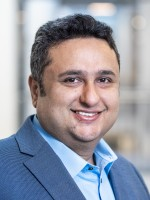
\includegraphics[height=1.5in,width=1in,clip,keepaspectratio]{images/authors/saad.jpg}}
\noindent {\bf Saad Mubeen}\
Dr. Mubeen is an Associate Professor at Mälardalen University, Sweden. He has previously worked in the vehicle industry as a Senior Software Engineer at Arcticus Systems and as a Consultant for Volvo Construction Equipment, Sweden. Dr. Mubeen is a Senior Member of IEEE. He is a Co-chair of the Subcommittee on In-vehicle Embedded Systems within the IES Technical Committee on Factory Automation. His research focus is on model- and component-based development of predictable vehicle software, modeling and timing analysis of in-vehicle communication, and end-to-end timing analysis of distributed embedded systems. Within this context, he has co-authored over 125 publications in peer-reviewed international journals, conferences and workshops. He has received several awards, including the IEEE Software Best Paper Award in 2017. He is a PC member and referee for several international conferences and journals respectively. He is a guest editor of IEEE Transactions on Industrial Informatics (TII). He has co-organized several special sessions at the international conferences such as IEEE IECON and ICIT.  He has also organized the 9th International Workshop on Compositional Theory and Technology for Real-Time Embedded Systems (CRTS 2016) and Model-based Engineering of Cyber Physical Systems track at the 13th International Conference on Information Technology: New Generations (ITNG), 2016.}
\vspace{4\baselineskip}

\bibliographystyle{IEEEtran}
\bibliography{IEEEabrv,main.bib}

% \bibliographystyle{unsrt}
% \bibliography{./main.bib}

\end{document} 